
%% Template Elsevier for Neuroimage

%% Use the option review to obtain double line spacing
%\documentclass[authoryear,preprint,review]{elsarticle}
\documentclass[authoryear]{elsarticle}
%\usepackage[framed,numbered,autolinebreaks,useliterate]{mcode}
\usepackage[framed,autolinebreaks,useliterate]{mcode}
\usepackage{natbib}
\usepackage{amsmath}
%\usepackage{lineno}
\usepackage{rotating}

\usepackage{hyperref}
\usepackage{amssymb}
\usepackage{amsfonts}


%\usepackage{algorithm2e}
%\usepackage{algorithmic}
%\usepackage{todonotes}
\usepackage{pdflscape}
\journal{Neuroimage}
\usepackage{color,transparent}
%\usepackage{color} 
%\pdfoptionpdfminorversion 6
\pdfminorversion=5

%\usepackage{graphicx}
%\usepackage{subcaption}
%\usepackage{mwe}
\usepackage{subfig}
\usepackage{caption}
%\usepackage{subcaption}
\usepackage{setspace}

\begin{document}

% Title must be 150 words or less
\begin{frontmatter}
%\title{Feasibility of multi-centric fMRI connectivity studies of Alzheimer's disease}
%\title{Feasibility of multi-centric fMRI connectivity and impact }

%\title{Measurement bias and statistical power in multi-centric resting-state fMRI connectivity}
\title{Statistical power and measurement bias in multi-centric resting-state fMRI connectivity}


%\title{A power analysis for multisite studies in resting-state functional connectivity, with an application to clinical trials in Alzheimer's disease}

\author[a,b]{Christian~Dansereau}
\author[c]{Celine~Risterucci}
\author[c]{Emilio~Merlo Pich}
\author[d]{Douglas~Arnold}
\author[a,b]{Pierre~Bellec\corref{cor1}}
\ead{pierre.bellec@criugm.qc.ca}
\cortext[cor1]{Corresponding author}
\address[a]{Centre de Recherche de l'Institut Universitaire de G\'eriatrie de Montr\'eal, Montr\'eal, CA}
\address[b]{D\'epartement d'Informatique et de recherche op\'erationnelle, Universit\'e de Montr\'eal, Montr\'eal,CA}
\address[c]{F. Hoffmann-La Roche Ldt., Basel, Switzerland}
\address[d]{NeuroRx, Montreal, Quebec, Canada}

% Please keep the abstract between 250 and 300 words
\begin{abstract}


\end{abstract}

%-- 
\begin{keyword}
multisite \sep multiprotocol \sep bias \sep statistical power \sep sample size \sep resting-state \sep fMRI, connectivity
%fmri \sep effect size \sep multisite \sep clinical trial \sep AD biomarker
\end{keyword}
\end{frontmatter}

% Unique number for each line
%\linenumbers
%\listoftodos

\section*{Highlights}

\begin{itemize}
\item etc
 %\item The impact of the number of nodes, or scale, on the sensitivity of a connectome-wide association study is systematically evaluated.
 %\item A procedure is presented that controls the false-discovery rate within- and between scales.
 %\item The technique is evaluated on a simulation of multiscale changes in connectome organization.
 %\item The technique is applied on three different datasets, for which there is a good a priori knowledge on the underlying connectivity changes.
 %\item Several recent procedures for connectome-wide association are compared.
\end{itemize}

\section{Introduction}
%Resting-state (RS) connectivity in fMRI is a promising biomarker for a variety of neurological diseases. Typically, in a clinical trial, a large cohort is recruited and evaluated at multiple sites spread over countries or even continents. In academia the budget allowed per investigator for scanning is generally of the order of 30 to 50 subjects leading to small cohorts, one problem with small sample size is the difficulty to detect small and consistent effect (differences) between groups. A solution that can help on this front is to increase the number of subject by pooling small RS cohorts acquired on the same scanner or on different scanners, this approach is referred to has multisite acquisition.


% Magic paragraph
Resting-state (RS) connectivity in fMRI is a promising biomarker for a variety of neurological diseases. Although, there is increasing concern about the reliability and reproducibility of scientific research and findings. One major source of concern within neuroscience is the low statistical power of many published studies, given that this increases the proportion of published findings that are false and can create unwanted biases or difficulty to detect small and consistent effect (differences) between groups. These worries have increased pressure to amass larger samples, but in many cases this is not feasible due to recruitment constraints (for example, when the number of subjects with a particular disorder in any geographical area is limited) or financial limitations. A solution to that problem is to increase the number of subject by pooling small RS cohorts acquired on the same scanner or on different scanners, this approach is referred to has multisite acquisition. Multi-site study are more and more common in fMRI and a lot of initiative have started to emerge to provide public data acquired at multiple sites. Has reported by \cite{Cheng2015} there is an urgent need to use methods that will allow large-scale pooling of data to both reduce the impact of heterogeneity between studies and allow the study of stratified subgroups. Nevertheless, multi-centric studies come with there share of advantages and disadvantages. The main advantages are the rapid recruitment of large sample-size across multiple sites and potentially distant geographically. This parallel recruitment provide better generalization due to more diversity in the scanners used although result in potential new sources of variance. This bias in measurement originating from the various acquisitions sites may decrease the benefit of a large sample-size due to the added variability in the data. We are therefore taking advantage of a public fMRI resource that incorporate these kind of variabilities to address this question and several others.

% Poldrack
%Reducing the cost of doing science. Making data available can greatly reduce the cost of scientific research when those data are relevant to new questions. Not all questions of interest can be answered using existing data sets, but to the degree that they can, the use of these shared data instead of collecting redundant new data could be a significant source of savings for researchers, allowing more money to be spent on personnel involved in data analysis.
\paragraph{Mutisite}
In most experiments conducted in neuroimaging, the main factors that influence power are: (1) the size of the effect, determined by the difference of the mean connectivity of one group versus a control group and the variability of this difference across subjects and groups; and (2) the sample size, i.e. the number of subjects in the study \citep{Desmond2002}. This last factor is usually the only one controlled by the investigator, hence why an increasing number of researchers share data. Multisite studies can be classified in two categories, the first one is independent studies that we would like to pool together even though the acquisition protocol are heterogeneous like the 1000 functional connectome project. The second category is the standardised studies across multiple sites, were a strict protocol is in place to harmonize the sites and an effort to homogenize the scanner parameters et acquisition protocols as been done like the ADNI dataset. Various reasons can justify multisite analysis, in research it is very difficult to obtain a grant large enough to scan a cohort larger than ~80 subjects, therefore researcher and consortium initiatives have started to pool their resources together to make initiative composed of publicly available large cohorts of subjects like the 1000 functional connectome \citep{Biswal2010}, ADNI \citep{Mueller2005}, among 
others. In clinical trial the justification for multicentric acquisition is more of a logistical one then a financial reason; they need to recruit a large amount of subject in a short period of time. In order to achieve this goal they mandate the recruitment to multiple clinical centers across the globe which accelerate the evaluation time of a drug. Although these centers may be similar by their scanner protocols, scanners will have difference in their software version, specific add-on to the scanners, and, most importantly, vendors (even field strength may differ in some cases). Unfortunately between studies, MR acquisition methodologies are among the most commonly cited sources of measurement variation \citep{Friedman2006}. This is why it is important to assess if multi-site resting-state connectivity analysis are feasible (we can combine the data from multiple sources while introducing a reasonable amount of variance which is still acceptable to detect effects in the data) and what corrective measure on the data should be applied to reduce the bias introduced by multisite analysis. 

%grosse etude multicentrique pour les grosse étude 
%CORR, ADHD200, INDI 
%(1000 functional connectome project, CORR, ABIDE, ...)
%datasharing d'étude multiple 


%\textbf{Difficulty of increasing the sample size}
%\begin{itemize}
%\item Collecting a large sample size is very expensive.
%\item Recruitment may be difficult at a single site.
%\item Large sample size can be achieved in multisite study.
%\item Multisite studies come with problems of their own.
%\end{itemize}


\paragraph{Sources of variance across sites}
%%\frametitle{Source of variance across sites}
%\begin{itemize}
%\item \textbf{Inclusion/exclusion criteria.}
%\item \textbf{Socio-cultural characteristics of recruiting sites} \\(e.g., ethnicity, language, diet, socioeconomic status).
%\item \textbf{Acquisition-related factors} \\(e.g., scanner make and model, sequence type, coil type, repetition time, flip angle, acquisition volume, etc).
%\item \textbf{Experimental design-related variations} \\(e.g., eyes-open/closed, experiment duration, instruction to participant).
%\item \textbf{Environmental-related variations} \\(e.g., sound, room temperature, head-motion restraint).
%\end{itemize}
%
%
%\textit{
%\begin{enumerate}
%\item Acquisition-related variations:
%\begin{enumerate}
%\item Scanner make and model \citep{Friedman2006}
%\item Sequence type (spiral vs. echo planar; single-echo vs. multi-echo) \citep{Klarhoefer2002}, parallel vs. conventional acquisition \citep{Feinberg2010} \citep{Lin2005}
%\item Coil type (surface vs. volume, number of channels, orientation).
%\item Acquisition parameters: repetition time, number of repetitions, flip angle, echo time, and acquisition volume (field of view, voxel size, slice thickness/gaps, slice prescription) \citep{Friedman2006a}.
%\end{enumerate}
%\item Experimental-related variations: 
%\begin{enumerate}
%\item Participant instructions \citep{Hartstra2011}, eyes-open/eyes-closed \citep{Yan2009} \citep{Yang2007}, visual displays, experiment duration \citep{Fang2007} \citep{VanDijk2010}.
%\end{enumerate}
%\item Environment-related variations: 
%\begin{enumerate}
%\item Sound attenuation measures \citep{Cho1998} \citep{Elliott1999}.
%\item Attempts to improve participant comfort during scans (e.g., music, videos) \citep{Cullen2009}.
%\item Head-motion restraint techniques (e.g., vacuum pad, foam pad, bite-bar, plaster cast head holder) \citep{Edward2000} \citep{Menon1997}.
%\item Room temperature and moisture \citep{Vanhoutte2006}.
%\end{enumerate}
%\end{enumerate}
%}

% Sources of variance
Beyond small sample sizes resulting in low statistical power \citep{Kelly2012a} and inconsistency in the results, there are other methodological differences that may compromise the comparison of results across independent studies. For example, the criteria for recruiting subjects may differ among studies. Different study samples may also reflect different socio-cultural characteristics of recruiting sites, e.g., ethnicity, language, diet, socioeconomic status. The fMRI measurements themselves can also be affected by differences in details of the image acquisition such as scanner make and model \citep{Friedman2006}, sequence parameters such as repetition time, flip angle, or acquisition volume \citep{Friedman2006a}, experimental design such as eyes-open/eyes-closed \citep{Yan2009} or experiment duration \citep{VanDijk2010}, and scanning environment such as sound attenuation measures \citep{Elliott1999}, room temperature \citep{Vanhoutte2006}, or head-motion restraint techniques \citep{Edward2000}. 
% Transition to the main question and the dataset used
Knowing that there is several sources of variance, the question is how much do they affect our analysis and does the trade-off of pooling datasets in exchange for increase variance and sample size worth it. Fortunately some resources exist that allow us to evaluate this question  empirically. 

\paragraph{Evaluation dataset} In 2009, the publicly released 1000 Functional Connectomes Project (FCP) and International Neuroimaging Data-sharing Initiative (INDI) provided a glimpse of the variability in imaging methodologies employed by the neuroimaging field. The dataset includes rs-fMRI samples independently collected at imaging sites around the world. A noteworthy aspect of this dataset is the variation in almost every parameter of the imaging acquisition methodologies, while the majority of subject-related variables are not reported (due in most cases, to the fact that they were not thoroughly recorded). 
Despite justifiable scepticism, feasibility analyses demonstrated that meaningful explorations of the aggregate dataset, composed of 24 imaging sites for a grand total of 1093 subjects, could be performed \citep{Biswal2010}. Although no explicit correction for multi-site variability was used, they only use global signal correction (GSC) to normalize subjects which may introduce anti-correlation in the data \citep{Fox2009, Murphy2009, Saad2012, Carbonell2014, Power2014}. After accounting for site-related differences, the analysis showed brain-behaviour relationships with phenotypic variables such as age, gender, and diagnostic label, and confirmed a variety of prior hypotheses \citep{Biswal2010, Fair2012, Tomasi2010, Zuo2012}. While encouraging, many uncontrolled and unknown factors in the 1000 FCP remain a source of concern, as they spread beyond simple site effects and can limit the datasets utility as highlighted by \cite{Yan2013}. An other compelling proof of multi-site bias is the study reported by \cite{Nielsen2013} where they did an analysis on a single site dataset and a multi-site dataset of subject with autism and concluded that the multi-site autism study classification accuracy significantly outperformed chance but was much lower for multi-site prediction than for previous single site results \citep{Nielsen2013}. We therefore need to keep in mind that the site effect must be taken in account in the analysis or we may reduce our detection power.


\paragraph{Specific objectives} 
The main potential issue with that approach is the lack of consistency in the multisite RS connectivity acquisitions that may obscure clinically relevant information. Therefore the aims of the study were to: (1) characterize the amplitude of the intra-site and inter-site connectivity bias, i.e. the systematic differences in rs-fMRI connectivity across different acquisition sites; (2) Quantify the impact of the inter-site variance on the detection power of a rs-fMRI effect. More specifically how sample size, group balancing and interaction of site-pathology in multi-centric topology impact sensitivity.

\section{Method}

\subsection{Data samples} 

\paragraph{Participants}
The paper studies 345 cognitively normal young adults (CNY) from the 1000 functional connectome project\footnote{\url{http://fcon_1000.projects.nitrc.org/}} (150 males, age range = 18-46 yrs) as a reference dataset. One of the particularity of this dataset is the presence of one large site of $\sim200$ subjects and 7 small sites of $\sim20$ subjects per site. We are therefore able to simulate realistic scenarios where we model the variability of a real monosite and the variability introduce by combining small sites into a large sample of the same total sample size, see Table \ref{table_dataset} for more details on each site. The experimental protocols for all datasets were approved by there respective ethic boards.


\begin{table}[tbp]
\resizebox{\columnwidth}{!}{%
\begin{tabular}{lllllllllll}
\textbf{Site}         & \textbf{Magnet} & \textbf{Scaner brand} & \textbf{Channels} & \textbf{N} & \textbf{N final} & \textbf{Sex} & \textbf{Age} & \textbf{TR} & \textbf{\# Slices} & \textbf{\# Frames} \\
Baltimore, USA        & 3T              & N/A                   & N/A               & 23   & 21         & 8M/15F       & 20-40        & 2.5         & 47                 & 123                \\
Berlin, Germany       & 3T              & Siemens Tim Trio      & 12                & 26   & 26         & 13M/13F      & 23-44        & 2.3         & 34                 & 195                \\
Cambridge, USA        & 3T              & Siemens Tim Trio      & 12                & 198  & 195        & 75M/123F     & 18-30        & 3           & 47                 & 119                \\
Newark, USA           & 3T              & N/A                   & N/A               & 19   & 17         & 9M/10F       & 21-39        & 2           & 32                 & 135                \\
NewYork\_b, USA       & 3T              & Siemens               & N/A               & 20   & 18         & 8M/12F       & 18-46        & 2           & 33                 & 175                \\
Oxford, UK            & 3T              & Siemens Tim Trio      & 12                & 22   & 20         & 12M/10F      & 20-35        & 2           & 34                 & 175                \\
Queensland, Australia & 4T              & Bruker                & 1                 & 19   & 17         & 11M/8F       & 20-34        & 2.1         & 36                 & 190                \\
SaintLouis, USA       & 3T              & Siemens Tim Trio      & 12                & 31   & 31         & 14M/17F      & 21-29        & 2.5         & 32                 & 127               
\end{tabular}
}
\caption{Site selected from the 1000 functional connectome dataset.} 
\label{table_dataset}
\end{table}

\paragraph{Acquisition} %Resting-state scans were acquired on a 3T Siemens TrioTim for all datasets. One single run was obtained per subject for either the SCHIZO or BLIND dataset while two runs were acquired in each subject for the MOTOR dataset, one immediately preceding and one following the practice on a motor task. 
%For the 1000 functional connectom dataset, 150 EPI volumes were recorded in 6 mins 40 s (TR = 2.65s, TE = 30ms, FA = 90\textdegree, 43 slices, voxel size = 3.4x3.4x3 mm$^3$, gap = 10\%, matrix size = 64x64, FOV = 220x220 mm$^2$), and a structural image was acquired using a MPRAGE sequence (TR = 2.3~s, TE = 2.98~ms, FA = 9\textdegree, 176 slices, voxel size = 1x1x1 mm$^3$, matrix size = 256x256, FOV = 256x256 mm$^2$).

We need to discuss how to present this data (I don't have the details for each site...)

\subsection{Preprocessing}\label{Preprocessing}
The datasets were analysed using the NeuroImaging Analysis Kit (NIAK\footnote{\url{http://www.nitrc.org/projects/niak/}}) version 0.12.14, under CentOS version 6.3 with Octave\footnote{\url{http://gnu.octave.org}} version 3.8.1 and the Minc toolkit\footnote{\url{http://www.bic.mni.mcgill.ca/ServicesSoftware/ServicesSoftwareMincToolKit}} version 0.3.18. Analyses were executed in parallel on the "Mammouth" supercomputer\footnote{\url{http://www.calculquebec.ca/index.php/en/resources/compute-servers/mammouth-parallele-ii}}, using the pipeline system for Octave and Matlab \citep{Bellec2010}, version 1.0.2. Brain map visualizations were created using MRICron software \cite{Rorden2007}. Each fMRI dataset was corrected of inter-slice difference in acquisition time and the parameters of a rigid-body motion was estimated for each time frame. Rigid-body motion was estimated within as well as between runs, using the median volume of the first run as a target. The median volume of one selected fMRI run for each subject 
was 
coregistered with a T1 individual scan using Minctracc \citep{Collins1998}, which was itself non-linearly transformed to the Montreal Neurological Institute (MNI) template \citep{Fonov2011} using the CIVET pipeline \citep{Zijdenbos2002}. The MNI symmetric template was generated from the ICBM152 sample of 152 young adults, after 40 iterations of non-linear coregistration. The rigid-body transform, fMRI-to-T1 transform and T1-to-stereotaxic transform were all combined, and the functional volumes were resampled in the MNI space at a 3 mm isotropic resolution. A censoring method described in \citep{Power2012} called "scrubbing" was used to remove the volumes with excessive motion using a cut-off value of $FD\geq0.5$. A minimum number of 50 unscrubbed volumes per run, corresponding to $\sim 125$ s of acquisition for a TR of 2.5 seconds, was then required for further analysis. The following nuisance parameters were regressed out from the time series at each voxel: slow time drifts (basis of discrete cosines 
with a 0.01 Hz high-pass cut-off), average signals in conservative masks of the white matter and the lateral ventricles as well as the first principal components (95\% energy) of the six rigid-body motion parameters and their squares \citep{Lund2006},\citep{Giove2009}. The fMRI volumes were finally spatially smoothed with a 6 mm isotropic Gaussian blurring kernel. 


\subsection{Functional networks}

\paragraph{Functional parcellation}
Regions are routinely defined using an anatomical parcellation \citep{He2009}, such as the AAL template \citep{Tzourio-Mazoyer2002}. Anatomical parcels may however not well match the brain functional organization. In this work, we used functional brain parcellations, aimed at defining groups of brain regions with homogeneous time series. A number of algorithms have been proposed with additional spatial constraints, to ensure that the resulting parcels are spatially connected \citep{Lu2003,Thirion2006,Craddock2012}. We can achieve this aim and reduce the computational burden of the analysis using a region-growing algorithm \cite{Bellec2006},  resulting in more homogeneous regions composed of temporally similar and contiguous voxels. The spatial dimension was selected arbitrarily by setting the size where the growing process stopped (a threshold of 1000 mm3 resulted into R=957 regions) from a reference dataset of healthy adults from the 1000 functional connectome project (Cambridge cohort \citep{Biswal2010}, parcellation available here \ref{}). The regions were built to maximize the homogeneity of the time series within the region, i.e. the average correlation between the time series associated with any pair of voxels of the region. The region growing was applied on the time series concatenated across all subjects (after correction to zero mean and unit variance), such that the homogeneity was maximized on average for all subjects, and the small homogeneous regions are identical for all subjects. Because of the temporal concatenation of time series, we had to limit the memory demand, and the region-growing was thus applied independently in each of the 116 areas of the AAL template \citep{Tzourio-Mazoyer2002}. See \cite{Bellec2006} for more details regarding the implementation of the region-growing algorithm. Overall, this process reduced the dataset of each subject into a (T x R) data array, where T is the number of time samples and R is the number of regions.

\paragraph{Functional network decomposition}
From a pure functional viewpoint, the spatial constraint seems somewhat arbitrary, as functional units in the brain at low resolution encompass distributed networks of brain regions with homotopic regions often being part of a single parcel \citep{DeLuca2006,Damoiseaux2006}. Some works have thus used distributed parcels as the spatial units to measure functional brain connectivity, e.g. \citep{Jafri2007,Marrelec2008}. We relied on a recent method called “Bootstrap Analysis of Stable Clusters” (BASC), which can identify consistent functional networks for a group of subjects \citep{Biswal2010}. using a hierarchical cluster with Ward’s criterion both at the individual and the group levels. The functional networks can be generated at any arbitrary scale (within the range of the fMRI resolution), and we considered only networks generated at the group level, which were non-overlapping and not necessarily spatially contiguous. In the present work we generated a BASC decomposition in 100 networks.

TODO: cite the NATURE paper of Pierre Orban for parcelation and connections selection.

\paragraph{Functional connectome}
Using a brain partition of $R$ networks obtain from BASC procedure described in \cite{Bellec2010c}, and taking each pair of distinct networks $i$ and $j$, the between-network connectivity $y_{i,j}$ is measured by the Fisher transform of the Pearson's correlation between the average time series of the network. The within-network connectivity $y_{i,i}$ is the Fisher transform of the average correlation between time series of every pair of distinct voxels inside network $i$. The connectome $\mathbf{Y}=(y_{i,j})_{i,j=1}^R$ is thus a $R\times R$ matrix. Each column $j$ (or row, as the matrix is symmetric) codes for the connectivity between network $j$ and all other brain networks (full brain functional connectivity map). For a scale with $R$ parcels, there are exactly $L=R(R+1)/2$ distinct elements in an individual connectome $\mathbf{Y}$.

\subsection{Simulations}

In order to simulate various scenarios within the context of a multi-site setting, a cohort of subjects acquired at a single-site was selected to act as our reference dataset and for the multi-site configuration a cohort from a collection of small sites, roughly totalling the same sample size as the reference dataset, was used. The simulation was based on a scenario with 8 sites for a total of 345 subjects, and no homogenization of acquisition protocol whatsoever. The multi-site (with correction) is based on 150 subjects from 7 sites and the monosite is based on one site of 195 subjects.  

\paragraph{Data generation process}
The following data generation model was used to test our hypothesis and estimate how the connectivity bias affect our ability to detect effects at the group level.
A sub-sampling procedure was performed on the datasets (monosite and multisite) previously described to obtain multiple samples. For each of the sample a Monte-Carlo simulation was implemented to evaluate the power of a resting-state multi-site study. For each site and each sample, a ratio $W$ of subjects were randomly assigned to a 'treatment' group, this ratio $W$ is referred to as the allocation ratio of participants. For the subjects in this group, a value was added to achieve a given relative effect size (Cohen's d, i.e. the mean of the two groups divided by the standard deviation of all sites). The study was repeated for various effect sizes (0 to 1.5 with a step of 0.01) on 11 connections based on the literature review previously described in (TODO: cite the NATURE paper of Orban2015) reporting reproducible pair of regions reported to be affected by Alzheimer disease progression and displayed connectivity changes between cognitively normal subjects and patient with dementia of the Alzheimer type.

\paragraph{multi-site correction approach} 
In order to obtain an unbiased method to combine sites and do group analysis on them we are using dummy variables (binary vectors $1\times S$) who code for each site in the GLM model illustrated in Equation\ref{eq_glm_dummy}. The variables are corrected to have a zero mean across subjects, and an intercept (i.e. a column filled with 1) is added to $\mathbf{X}$. The GLM relies on the following stochastic model:

\begin{equation}
 \label{eq_glm_dummy}
  \mathbf{Y} = \mathbf{X}\mathbf{\beta} + \mathbf{V}\mathbf{\gamma}+ \mathbf{E},
\end{equation}
\begin{itemize}
  \item $\mathbf{Y}$: $N\times 1$, connectivity value for the pair ($i,j$),
  \item $\mathbf{X}$: $N\times K$, explainable variables,
  \item $\mathbf{\beta}$: $1 \times K$, regression values for each explainable variable,
  \item $\mathbf{V}$: $N\times S$, each column code for a site (0/1),
  \item $\mathbf{\gamma}$: $1\times S$, site average connectivity,
  \item $\mathbf{E}$: $N\times 1$, residual values from the regression,
\end{itemize}
 
with $N$ the number of subjects, $K$ the number of explainable variables and $S$ the number of sites. Where $\mathbf{\beta}$ is an unknown $1\times K$ vector of linear regression coefficients, $\mathbf{\gamma}$ is a $1\times S$ vector of linear regression coefficients representing the contribution of each site and $\mathbf{E}$ is a $N\times 1$ random (noise) multivariate Gaussian variable. As data generated from different subjects are statistically independent, and under an homoscedasticity assumption, the regression coefficients $\mathbf{\beta}$ can be estimated with ordinary least squares. To apply the correction $S-1$ dummy-variables are added to the model in Equation\ref{eq_glm_dummy} with $S$ being the total number of sites used in the study.


% list of parameters for generation (connections, effect-size, sample size, )
The parameters that we are manipulating in this study depend on the scenario 

% statistical detection and sensitivity
\paragraph{Statistical detection  and sensitivity}
The following confounding variables were modelled in the general linear model (GLM) analysis: frame displacement (FD). Significance of the results is obtain with a Student $t$-test and the sensitivity of the test is evaluated by sub-sampling 70\% of the dataset ($B=10^3$ random samples). For each sample $b$, we have a $p$-value $p^{*}_b$ and the detection sensitivity is estimated by the probability of $p^{*}_b$ being inferior to $0.001$.
\begin{equation}\label{Detection power}  
    \frac{1}{B}\sum\limits_{b=1}^B\left(p^{*}_b\leq0.001\right).
\end{equation}

To account for site-specific bias we have included dummy variables in the GLM model as well as confounding variable to account for age, sex and frame displacement (FD). The significance of the difference between the control and 'treatment' group was assessed by a $t$-test in a linear model.

% homoscedastic hypo (voir glm-connectome revision 2 sur svn)

We relied on the following parametric assumptions on the noise E (1) that its rows are independent; (2) that each element follows a normal distribution with zero mean, and (3) that the variance of all elements are constant within a column, also called the homoscedasticity assumptions. As the data generated from different subjects are statistically independent the first assumption is reasonable. We tested the normality and homoscedasticity assumptions on real datasets. Under these parametric assumptions, the regression coefficients B can be estimated with ordinary least squares and, for a given “contrast” vector c of size 1 × C, the significance of cBˆ 167 can be tested with a connectome of t-test

(tl)^{L}_{l=1}, with associated p-values (pl)



l=1 168 . The quantity pl controls for the risk of false positive findings at each connection l. The GLM applied on connectomes is illustrated in Figure 1c. See Appendix B for the equations related to the estimation and testing of regression coefficients in the GLM.



% the scenarios and the 3 sections
We first evaluated if a bias can be detected between sites. To do so we have computed the average connectome of each site along with the standard deviation matrix for each site. We then computed the statistically significant differences between each sites (FDR correction XX, ttest at p<XX) to have an idea of the size and spread of the functional bias.





\paragraph{Effect size (cohen's d)}
For each site and each sample, half of the subjects were randomly assigned to a "treatment" group and a Monte-Carlo simulation was used to estimate the detection power in the single-site and in multi-site setting.

The normalized Cohen's d was used to estimate the effect size and it is defined as the difference between two means $\bar{x_{1}},\bar{x_{2}}$ divided by a standard deviation from the data $s$.

For each site an effect is added to the connectivity of $B\%$ of the subjects, selected randomly ("pathological" group):
\begin{equation}
	y_{i,j} = y_{i,j} + \mu.
\end{equation}

The parameter $\mu$ is chosen to obtain a particular effect size (measured by the Cohen $d$)
%The normalized Cohen's d was used to estimate the effect size and it is defined as the difference between two means $\bar{x_{1}},\bar{x_{2}}$ divided by a standard deviation from the data $s$.
\begin{equation}\label{cohen's d}
    \begin{array}{l l}
      d = \frac{\mu}{s_{i,j}},      
    \end{array}
\end{equation}
where $s_{i,j}$ is the standard deviation between region $i$ and $j$ for the reference population (mono-site, Cambridge). The significance of the difference between the control and 'treatment' group was assessed by a $t$-test in a linear model, including a covariate to model the motion. The study was repeated for various effect sizes (0 to 0.8 with a step of 0.01) with a $p$-value threshold of $0.001$ on the $t$-test.

In order to introduce the same effect-size across the single-site and multi-site dataset we are taking the standard deviation from the single-site cohort as the reference.  The connection $y_{i,j}$ of the randomly affected subjects ("treatment" group) are therefore calculated $y_{i,j} = y_{i,j} + d\times s_{i,j}$. 




 
% The second approach is to compute the GLM independently on each site and then combine the statistical results from each site in a global score. This model averaging technique called METAL from \cite{Willer2010} model site specific bias by running a GLM analysis on each site resulting in $v$ beta vectors that are weighted proportionally to the standard error of each site and finally averaged as shown in equation \ref{METAL}. This is the most flexible way to account for multi-site effect wile keeping the analysis simple and robust to unbalanced sites.
% 
% \begin{equation}
% 	\beta_{v} \text{, effect size estimate for site \textit{v}.}
% \end{equation}
% \begin{equation}
% 	\sigma_{v} \text{, standard error for site} \textit{v}.
% \end{equation}
% \begin{equation}
%  	w_{v}=\frac{1}{\sigma_{v}^{2}} \text{, weight estimate for site \textit{v}.}
%  \end{equation}
%  \begin{equation}
%  	\beta=\frac{\Sigma_{v}\beta_{v}w_{v}}{\Sigma_{v}w_{v}} \text{, global }\beta.
%  \end{equation}
%   \begin{equation}
%  	\sigma=\sqrt{\frac{1}{\Sigma_{v}w_{v}}} \text{, global standard error.}
%  \end{equation}
% \begin{equation}\label{METAL}
% 	Z=\frac{\beta}{\sigma} \text{, global Z score.}
% \end{equation}
% \begin{equation}
% 	p=2(1-\phi(\vert Z \vert) \text{, p-value.}
% \end{equation}



%\paragraph{Framewise displacement (FD)}
%Index measure of head motion from one frame to the other. It is calculated as the sum of the absolute values of the differentiated realignment estimates at every time point \citep{Power2012} this measure give us an approximation of the motion frame by frame in millimeter. We are using this measure as an index of motion estimation.
%
%\begin{equation}
%    FD_{i} = \vert \triangle d_{x}(t) \vert + \vert \triangle d_{y}(t) \vert + \vert \triangle d_{z}(t) \vert + \vert \triangle r_x(t) \vert + \vert \triangle r_y(t) \vert + \vert \triangle r_z(t) \vert,
%\end{equation}
%\begin{equation}
%  r_x(t) = 50\left(\frac{2\pi\alpha_x(t)}{360}\right),
%\end{equation}
%with 
%\begin{itemize}
% \item ($d_x(t),d_{y}(t),d_{z}(t)$) translation parameters (mm),
% \item ($\alpha_x(t),\alpha_y(t),\alpha_z(t)$) rotation parameters (degres),
% \item $\triangle$ difference between time $t$ et $t-1$.
%\end{itemize}


\section{Results}

%The Figure \ref{fig_icc} presents the results of the ICC analysis for the point-to-point correlations, 
%(a), regional clustering (b), regional degree centrality (c), global summary such as the average clustering, average efficiency and modularity (d) and local efficiency (e). 
%only the connections with an average ICC above 0.5 are represented. The results were consistent with \citep{Shehzad2009}, with a mean ICC over all connections of \textasciitilde0.3 and 23 connections scoring a moderate-to-good level of ICC ($>0.5$). 

%In total, the literature review identified 7 nodes in the DMN (21 point-to-point correlations within the DMN) and 9 seeds in networks outside of the DMN (63 point-to-point correlations between a node in the DMN and a node outside of the DMN). We included three local network properties in the DMN (21 measures), as well as two global properties. That's a total of 107 candidate measures, based on a fairly conservative literature review. We further analyzed the test-retest reliability of these measures to narrow the selection down to about 10 measures. 

%The literature on TRT reliability of graph measures is much more difficult to interpret: \cite{Braun2012} for example has included many possible strategies to generate graph properties, resulting into almost the full range of possible ICC values for every metric ! Because no processing strategy was an obvious winner across all metrics, we selected the middle thresholding (20\% density) of \cite{Braun2012}. The relatively low ICC for graph measures (only a few measures with $ICC>0.5$, many measures with $ICC < 0.2$), was consistent with the results of \citep{Wang2011}.
% 
% \begin{table}[H]
% \begin{center}
% \begin{tabular}{l l l l}
% \bfseries{Network} & \bfseries{Label} & \bfseries{Name} & \bfseries{Cambridge100}\\
% \hline
%  & PCC & posterior cingulate cortex & 1\\
%  & dMPFC & dorsomedial prefrontal cortex & 12\\
%  & dMPFC2 & dorsomedial prefrontal cortex & 46\\
% Default-mode network & aMPFC & anterior medial prefrontal cortex & 42\\
%  & IPL & inferior parietal lobule & 49\\
%  & PCUN & precuneus & 53\\
%  & MTL & medial temporal lobe & 39\\
%  & SFGr & right superior frontal gyrus & 76\\
% \hline
% Visual network & FUS & fusiformgyrus & 71\\
% \hline
% Dorsal attentional & PCUMm & precuneus (motor) & 94\\
% \hline
% Cingulo-opercular network & dMPFC3 & dorsmedial prefrontal cortex & 90\\
% \end{tabular}
% \end{center}
% \caption{Regions selected in the literature review, the region number correspond to the number in the Cambridge 100 partition.}
% \label{tab_point-to-point}
% \end{table}
% 
% For point-to-point correlations within the DMN, we selected the connections with highest ICC for each node (all average ICC > 0.5):
% \begin{itemize}
% \item PCC x PCUN
% \item dMPFC x dMPFC2
% \item IPL x SFGr
% \item aMPFC x PCUN
% \end{itemize}
% For each point-to-point correlation between the DMN and another network, we selected the connections with highest ICC and ICC > 0.5:
% \begin{itemize}
% \item FUS x SFGr
% \item PCC x PCUNm
% \item IPL x dMPFC3
% \end{itemize}
% The only graph properties that satisfied the above criteria were:
% \begin{itemize}
% \item[•] average clustering
% \item[•] clustering PCUN
% \item[•] local efficiency PCUN
% \end{itemize}

\subsection{Inter-site variability}
The first assessment perform on the dataset was to verify the distribution of the variance in functional connectivity among each site and across sites in order to see if they are of the same order of magnitude or not. This analysis of Figure \ref{fig_site_variability} shows the distribution of the standard deviation in connectivity across subjects (the distribution is over the full brain connectome, with several 1000s connections) at the 8 sites against the inter-sites standard deviation of connectomes (average at each site). As we can see the inter-site (between-site) variability is smaller than the intra-site (between subjects) variability, in fact the amplitude of inter-site bias is about 3-fold smaller than the within-site standard deviation (red $\sim 0.06$ vs. orange $\sim 0.18$).

\begin{figure}[tbp]
\begin{center}
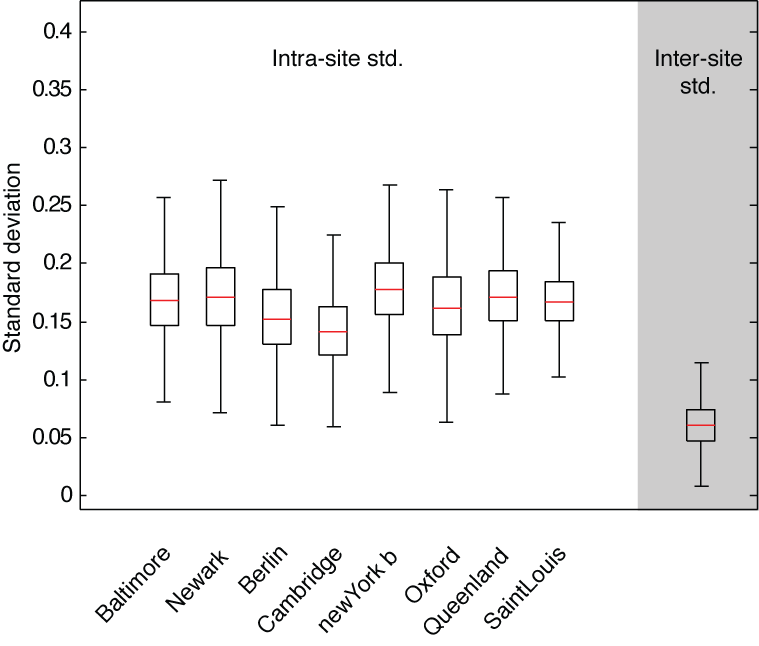
\includegraphics[width=\linewidth]{../figures/inter_vs_intra_3tonly.png}
\end{center}
\caption[inter vs. intra site variability]{
  Distribution of intra-site (between-subject) standard deviation vs. inter-site (between-site) standard deviation, based on the standard deviation of the connectivity matrices from 8 sites from the 1000 functional connectome dataset.
}
\label{fig_site_variability}
\end{figure}

In order to verify how spatial structure vary across sites the average standard deviation and the average connectivity map of the DMN were extracted for each site and reported in Figure \ref{fig_DMN_variability}. As we can see in the intersection between two sites the difference in average connectivity between-sites is illustrated (red set of brain cuts). First the mean DMN at each site is consistent with the expected spatial distribution reported in other studies \citep{Damoiseaux2006,Dansereau2014,Yan2013a}. The most salient changes between-sites are located in the mesio-frontal region associated with the anterior part of the DMN. In order to verify if significant changes are not only found in the DMN we have computed the entier connectome in order to obtain the other connectivity patterns and the findings can be generalized to the full connectome see Figure \ref{fig_connectome_variability}.

\begin{figure}[tbp]
\begin{center}
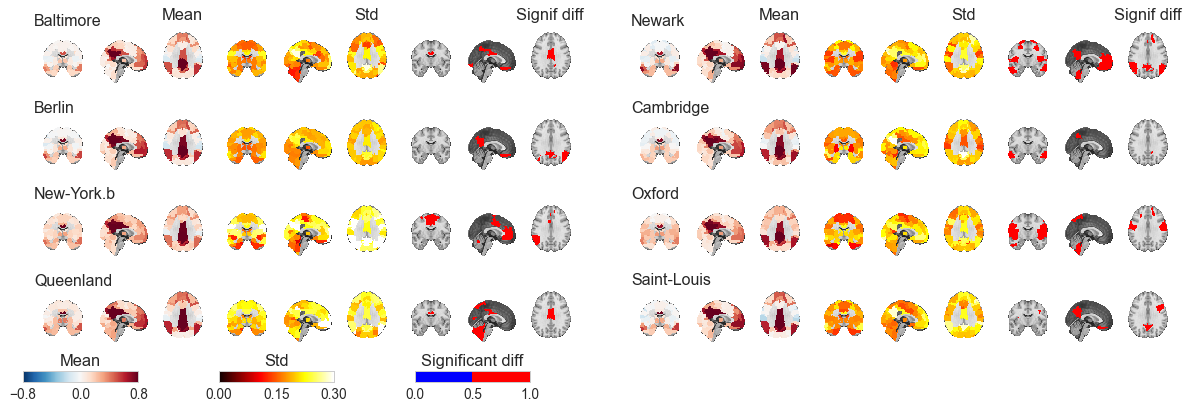
\includegraphics[width=\linewidth]{../figures/pccmap_multisite.png}
\end{center}
\caption[DMN variability across sites]{
Functional connectivity maps of the default-mode network at multiple sites. The average connectivity map are shown on the diagonal. The standard deviation across subjects and within site is shown on the first column. Each off-diagonal block represent the significant differences between the average functional connectivity maps between two sites (called the inter-site bias).
}
\label{fig_DMN_variability}
\end{figure}


\begin{figure}[tbp]
\begin{center}
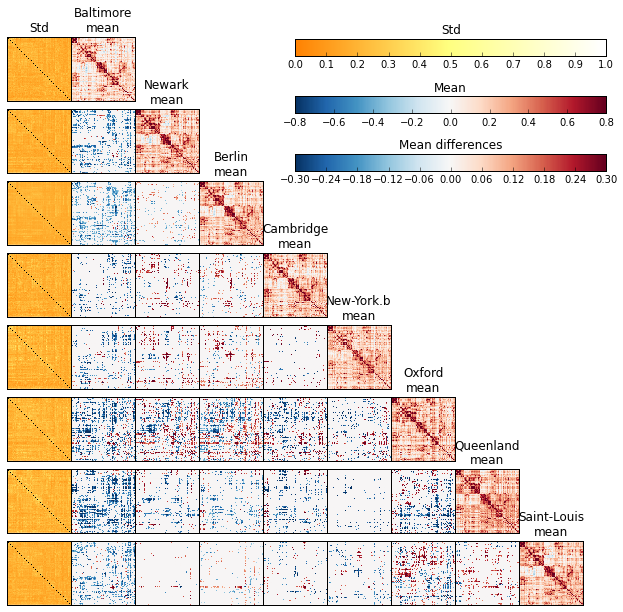
\includegraphics[width=\linewidth]{../figures/connectome_multisite.png}
\end{center}
\caption[Connectome variability across sites]{
Functional connectome for multiple sites. The average connectome of 8 sites (Baltimore, Newark, Berlin, Cambridge, New-Yorkb, Oxford, Queenland and SaintLouis at 3T) are shown on the diagonal. The standard deviation across subjects and within site is shown on the first column. Each off-diagonal block represent the absolute difference between the average functional connectivity maps between two sites (called the inter-site bias).
}
\label{fig_connectome_variability}
\end{figure}

\subsection{Simulation on real data}
% introduction of simulation intro the objectives...

In order to evaluate the impact of multisite configuration on our ability to detect changes in rs-functional connectivity studies we performed various simulation on real fMRI data. For each site and each sample, $B\%$ of the subjects were randomly assigned to a 'treatment' group. For the subjects in this group, a value was added to achieve a given relative effect size expressed in Cohen's d. The significance of the difference between the control and 'treatment' group was assessed by a $t$-test in a linear model. To account for site-specific bias we have included dummy variables in the GLM model. The study was repeated for various effect sizes (0 to 1.5 with a step of 0.01) at a threshold of 0.001 on the p-value.

Figure \ref{fig_p2p} show the pair of regions used in (TODO ORBAN2015) as candidate marker for functional connectivity changes in Alzheimer disease based on a literature review. We will use the correlation between those regions to estimate the variability across subject and induce some effect in our simulations.

\begin{figure}[tbp]
\begin{center}
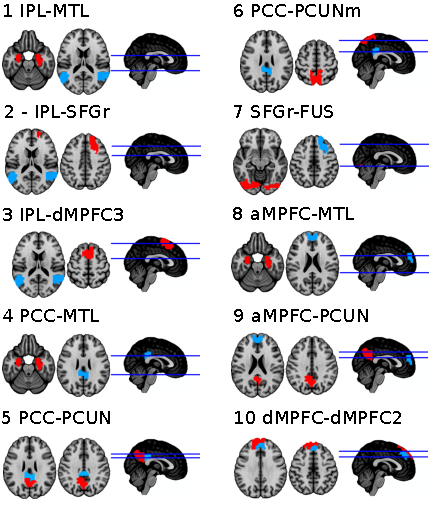
\includegraphics[width=0.5\linewidth]{../figures/p2p_seeds.pdf}
\end{center}
\caption{
Connexions pair based on a literature review.
}
\label{fig_p2p}
\end{figure}


In Figure \ref{fig_real_sim_samplesize} we show the effect of the sample size on the detection power. As expected we are able to detect smaller and smaller effect size as we increase the sample size. For an effect size of 1 which is considered a large effect we are able to detect significant changes in only 20\% of the cases at 40 subjects, 80\% at 80 subjects and almost 95\% at 120\% subjects.

%\frametitle{Effect of sample size: \\real data 50\%-50\% debalancing}
\begin{figure}[tbp]
\centering
\captionsetup[subfloat]{labelformat=empty}
\subfloat[][40 subjects]{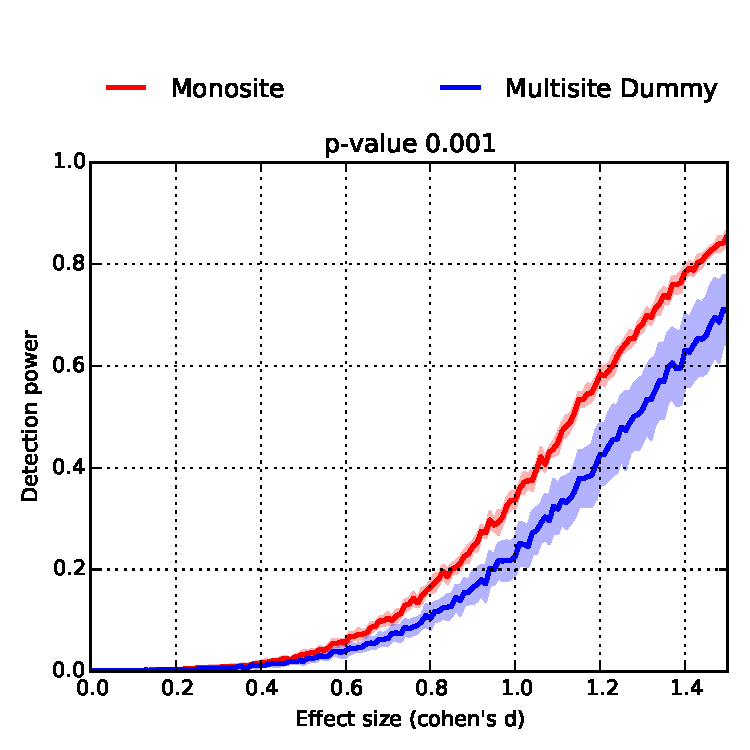
\includegraphics[width=0.32\textwidth]{../figures/realdata_detect_pow_s40_50pct.pdf}}
\hspace{1mm}
\subfloat[][80 subjects]{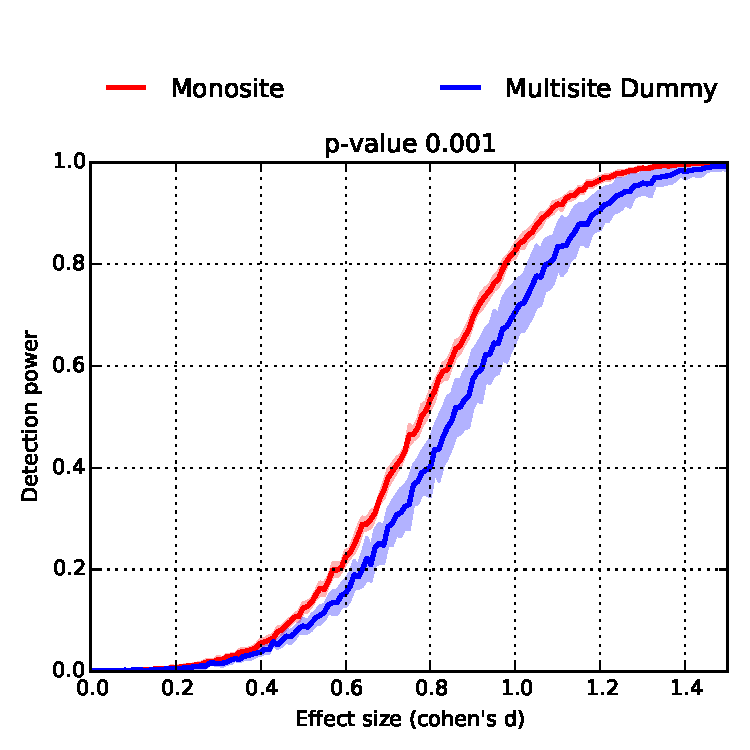
\includegraphics[width=0.32\textwidth]{../figures/realdata_detect_pow_s80_50pct.pdf}}
\hspace{1mm}
\subfloat[][120 subjects]{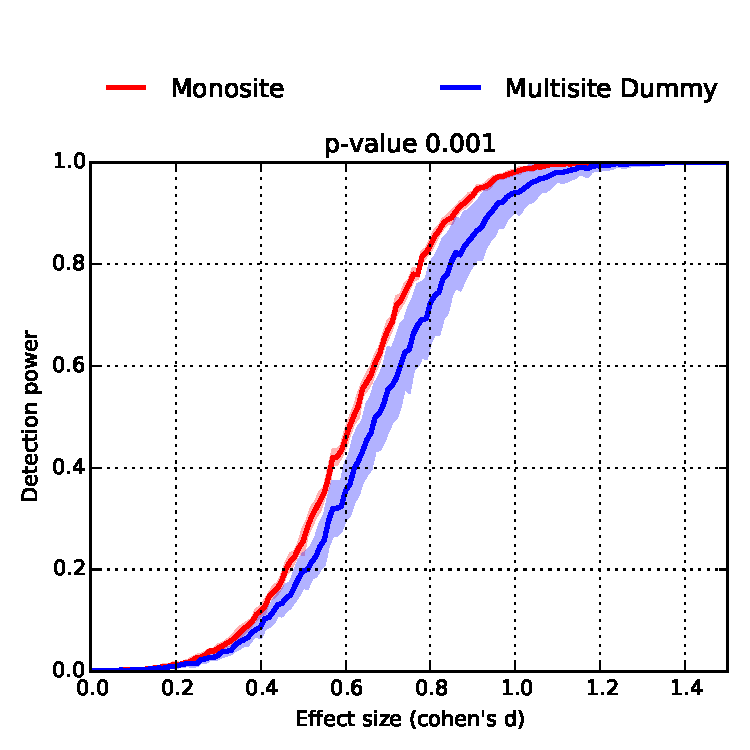
\includegraphics[width=0.32\textwidth]{../figures/realdata_detect_pow_s120_50pct.pdf}}
\hspace{1mm}
\caption{
Simulation on real data, detection power of two groups balanced 50\%-50\% between 7 sites. Two scenarios, 1) monosite and 2) multisite 7 sites with correction for multisite differences using dummy variables. Each plot show the detection power in function of the effect size for 3 different sample size 40, 80 and 120 subjects in total.
}
\label{fig_real_sim_samplesize}
\end{figure}

Figure \ref{fig_real_sim_debalancing} show the effect of debalancing the two groups at various ratio (50\%-50\% , 30\%-70\% and 15\%-85\%) for a total sample size of 120 subjects. Has the debalancing increase our ability to detect effect is diminished. As an example for an effect size of 1 we would detect the effect in 95\% of the cases in a 50 balanced scenario, this would go down to 90\% in a 30\%-70\% scenario and to 60\% in a 15\%-85\% debalancing. 


%\frametitle{Debalancing effect: \\real data 120 subjects total}
\begin{figure}[tbp]
\centering
\captionsetup[subfloat]{labelformat=empty}
\subfloat[][Debalancing 50\%]{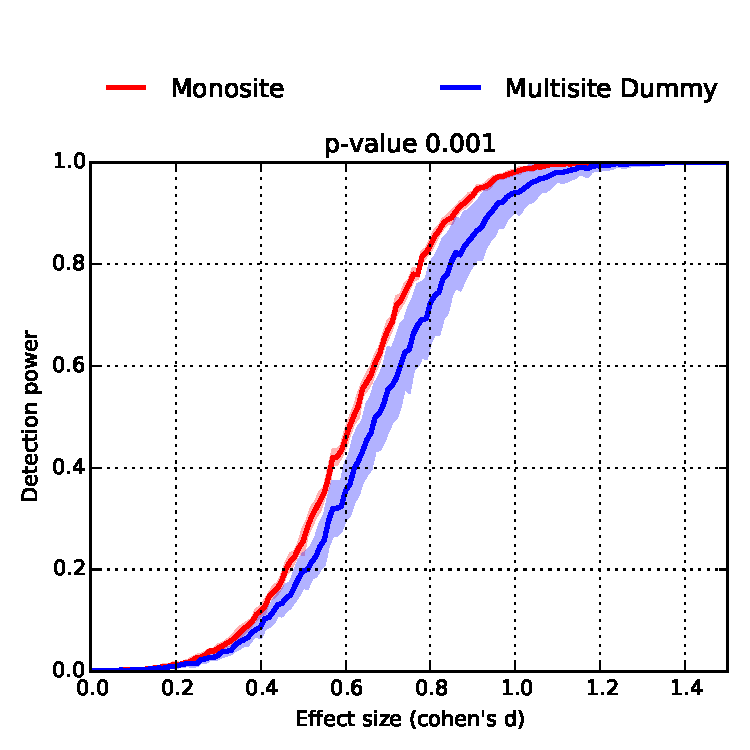
\includegraphics[width=0.32\textwidth]{../figures/realdata_detect_pow_s120_50pct.pdf}}
\hspace{1mm}
\subfloat[][Debalancing 30\%]{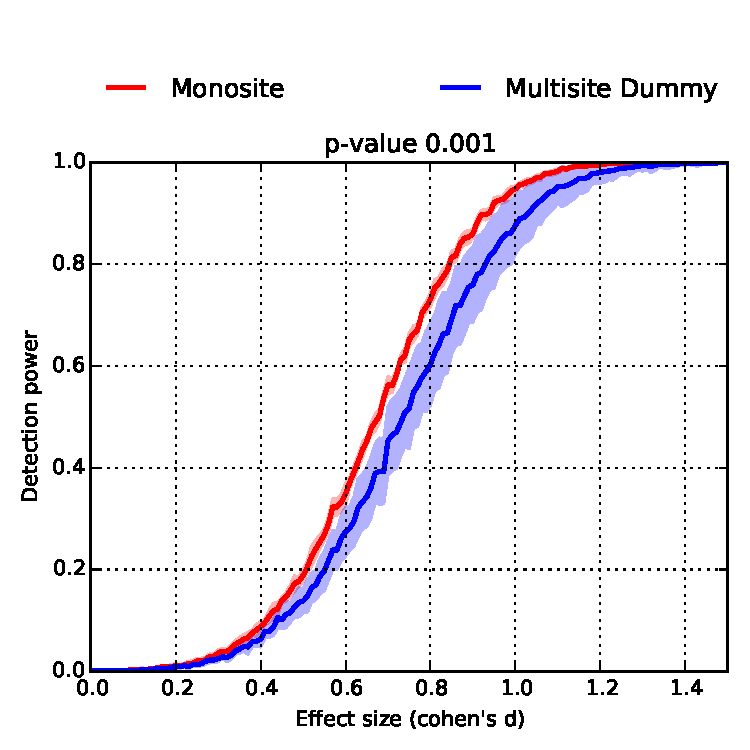
\includegraphics[width=0.32\textwidth]{../figures/realdata_detect_pow_s120_30pct.pdf}}
\hspace{1mm}
\subfloat[][Debalancing 15\%]{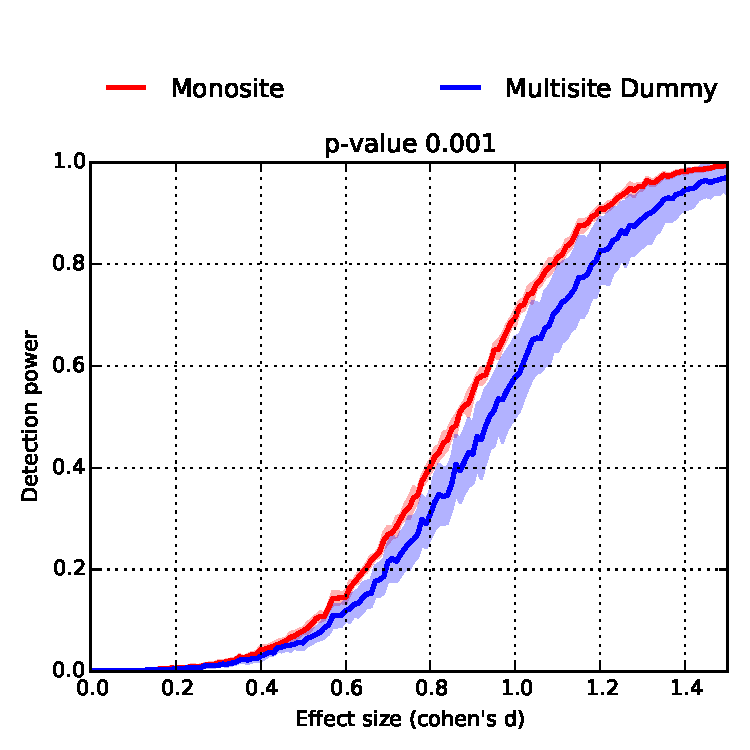
\includegraphics[width=0.32\textwidth]{../figures/realdata_detect_pow_s120_15pct.pdf}}
\hspace{1mm}
\caption{
Simulation on real data, detection power of two groups for a total of 120 subject between 7 sites. All plot show two scenarios, 1) monosite and 2) multisite 7 sites with correction for multisite differences using dummy variables.
}
\label{fig_real_sim_debalancing}
\end{figure}

Figure \ref{fig_real_sim_debalancing_interact} show the effect of debalancing the two groups at various ratio (50\%-50\% , 30\%-70\% and 15\%-85\%) with an interaction site-pathology (0.5 Cohen's d) for a total sample size of 120 subjects. Has the debalancing increase our ability to detect effect is diminished. As an example for an effect size of 1 we would detect the effect in 98\% of the cases in a 50 balanced scenario, this would go down to 95\% in a 30\%-70\% scenario and to 75\% in a 15\%-85\% debalancing. The particularity of this experiment is the fact that the multisite configuration perform better then the single site meanning that it is better to have interaction of various amplitude across small sites than an average interaction on one large site.


%\frametitle{Debalancing effect + interaction site-patho: \\real data 120 subjects total}
\begin{figure}[tbp]
\centering
\captionsetup[subfloat]{labelformat=empty}
\subfloat[][Debalancing 50\%]{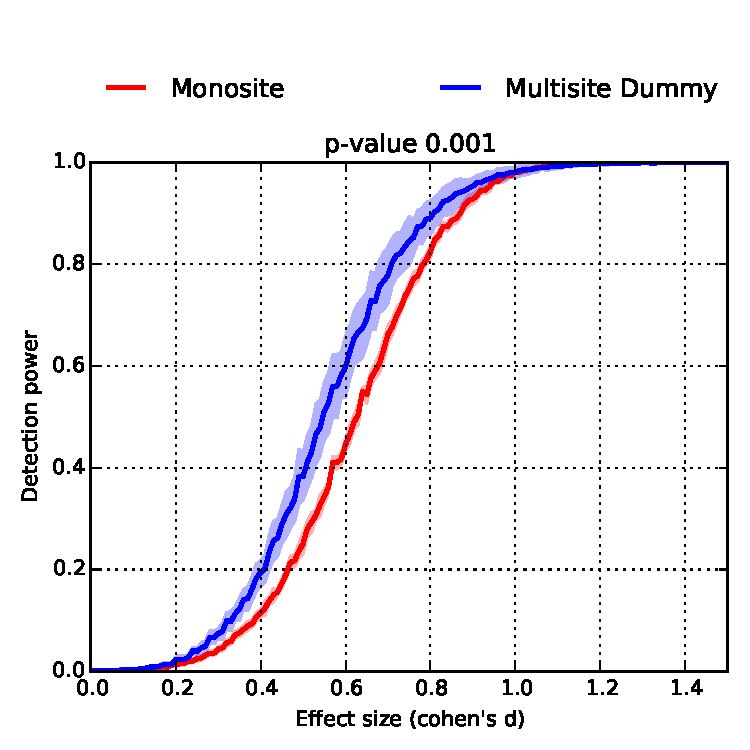
\includegraphics[width=0.32\textwidth]{../figures/realdata_detect_pow_sitepatho_s120_50pct.pdf}}
\hspace{1mm}
\subfloat[][Debalancing 30\%]{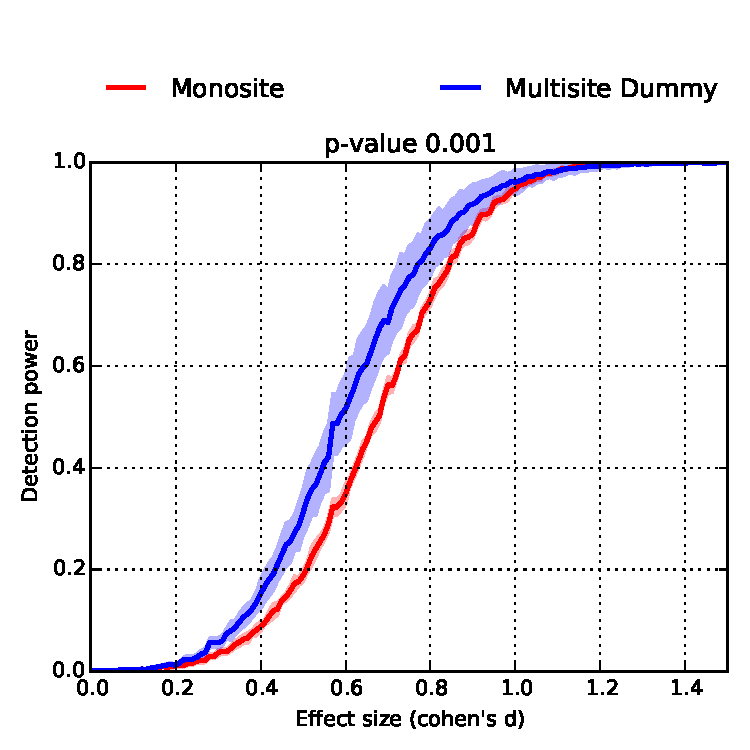
\includegraphics[width=0.32\textwidth]{../figures/realdata_detect_pow_sitepatho_s120_30pct.pdf}}
\hspace{1mm}
\subfloat[][Debalancing 15\%]{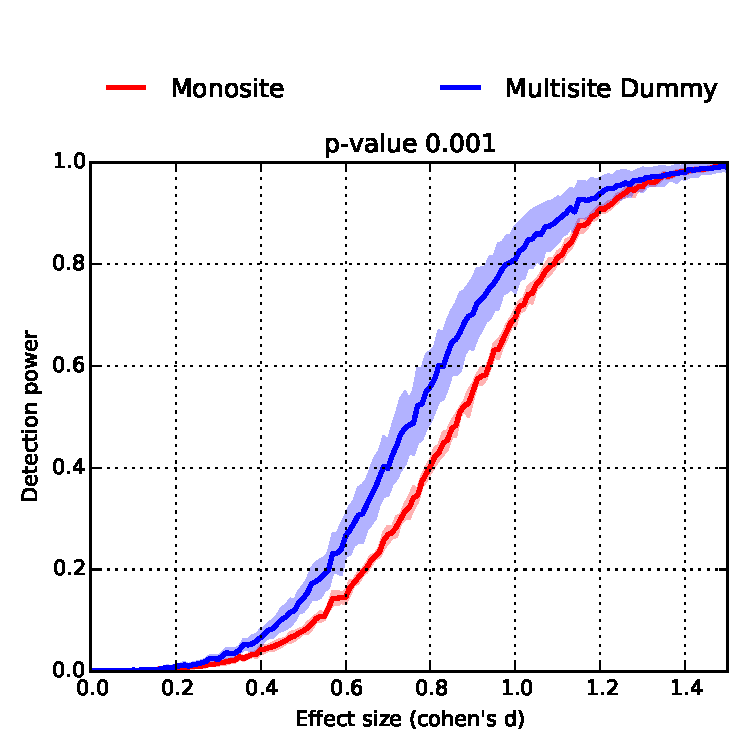
\includegraphics[width=0.32\textwidth]{../figures/realdata_detect_pow_sitepatho_s120_15pct.pdf}}
\hspace{1mm}
\caption{
Simulation on real data, detection power of two groups for a total of 120 subject between 7 sites with a site-pathology interaction at 0.5. All plot show two scenarios, 1) monosite and 2) multisite 7 sites with correction for multisite differences using dummy variables.
}
\label{fig_real_sim_debalancing_interact}
\end{figure}

Figure \ref{fig_real_sim_debalancing_2sites} show a scenario of two site one large (80 subjects) and one small ($\sim20$ subjects) unbalanced at 30\%-70\% and the inverse. As we can see the multisite configuration is as good as the monosite.

\begin{figure}[tbp]
\centering
\captionsetup[subfloat]{labelformat=empty}
\subfloat[\tiny 30\%-70\%]{\label{} 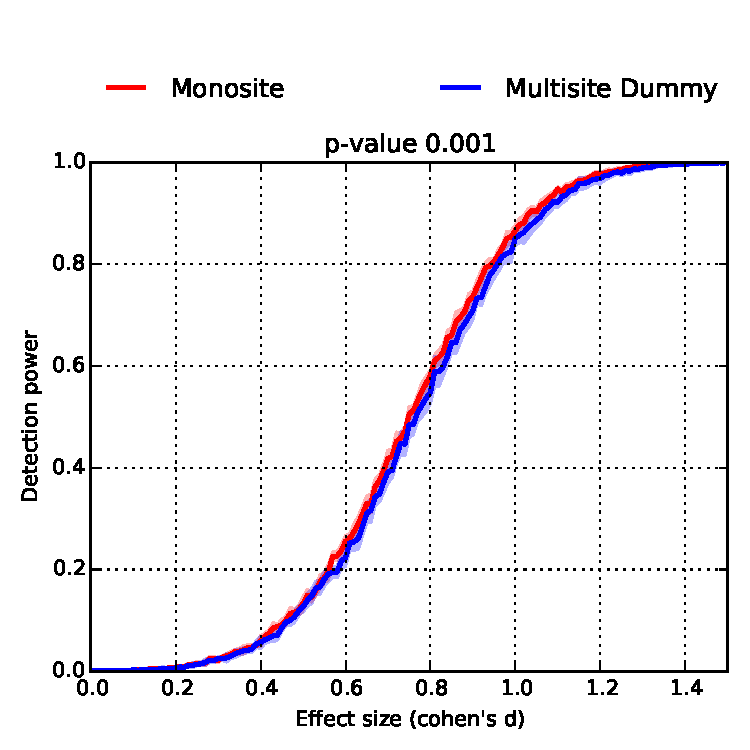
\includegraphics[width=0.39\textwidth]{../figures/realdata_detect_pow_sitepatho2site_s100_30pct.pdf}} 
\subfloat[\tiny 70\%-30\%]{\label{} 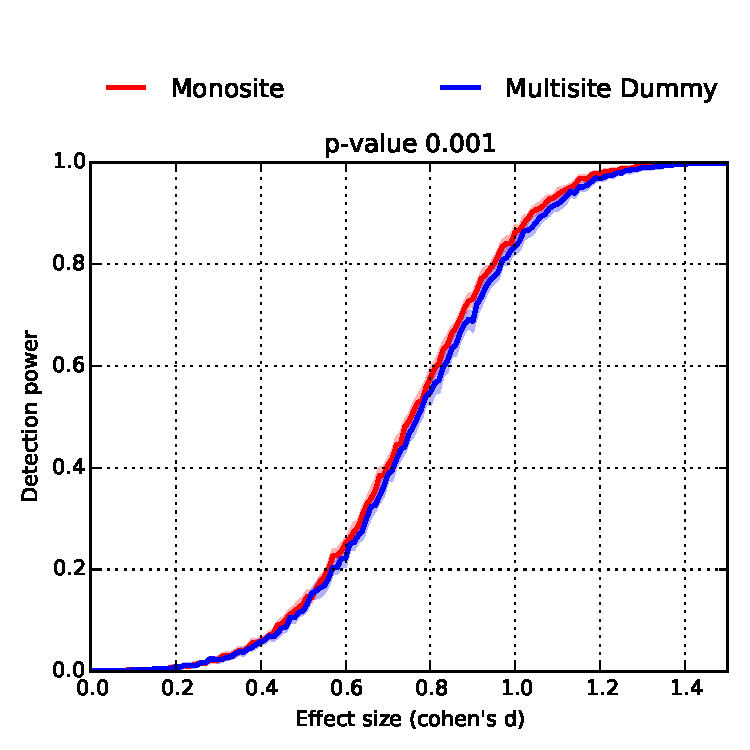
\includegraphics[width=0.39\textwidth]{../figures/realdata_detect_pow_sitepatho2site_s100_70pct.pdf}}\\
\caption{
Simulation on real data, detection power of two groups for a total of 100 subject between 2 sites, one small site of 20 subjects and one large of 80 subjects. All plot show two scenarios, 1) monosite and 2) multisite 2 sites with correction for multisite differences using dummy variables. Simulation of the detection power of two groups balanced 30\% and 70\% between 2 sites.
}
\label{fig_real_sim_debalancing_2sites}
\end{figure}

Using this Monte-Carlo simulations we have shown that the power of detecting an effect is marginally affected by the site acquisition configuration (single site or multi-site) when the sites are balanced in term of the amount of subject with and without the effect. 


\subsection{Simulation on synthetic data}
 
In order to obtain more control on each of the parameter of the simulation and simulate some configuration that were not possible to do with the real data (like the simulation of 2 medium size sites of of 40 and 60 subjects per site, and the size of the site effect) we have therefore used a synthetic model using only synthetic data and the average standard deviation of the Cambridge site connectivity. All plots show four scenarios: The top left plot represent the two configurations one monosite and two sites with correction for multisite differences using dummy variables without site effect. Has expected there is no difference between using 1 large site than combining two site of half the size. The plot on the upper right corner represent the detection power when we apply a site effect on balanced sites, here again not much differences an additive effect is fully compensated by the dummy variables corrective method. the lower left plot represent no site effect but an interaction between site and pathology. An the last plot on the lower right corner show the detection power with a site effect of 0.5 and a interation site pathology.

%\begin{frame} \frametitle{50-50 subjects, 50\%-50\% debalancing effect}
 \begin{figure}[tbp]
   \centering
    \captionsetup[subfloat]{labelformat=empty}
    \subfloat[]{ 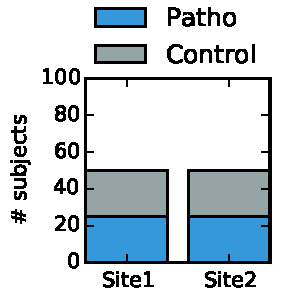
\includegraphics[width=0.19\textwidth]{../figures/prop_5050subj_5050.pdf}}
     \subfloat[\tiny No site effect]{ 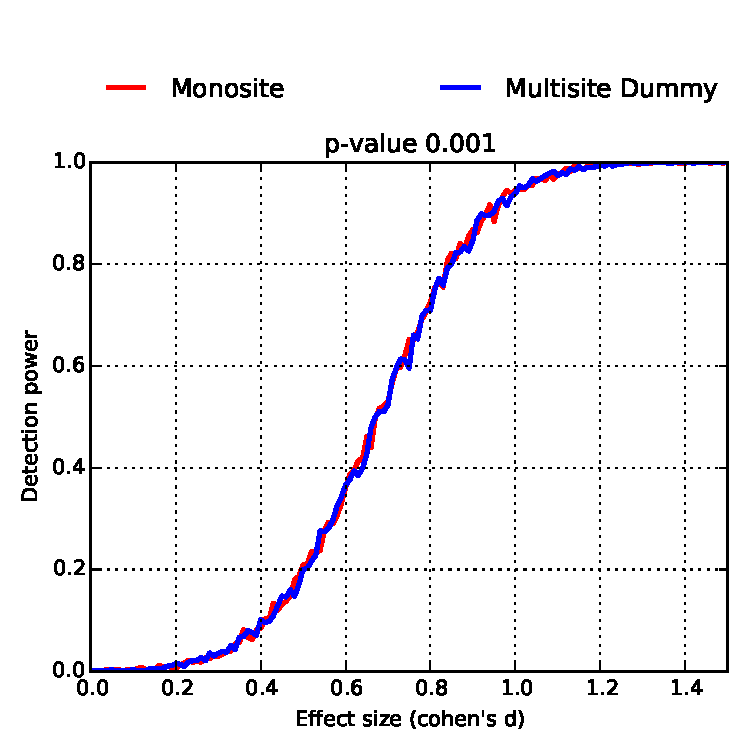
\includegraphics[width=0.39\textwidth]{../figures/detect_pow_bal5050_var0_site0.pdf}} 
     \subfloat[\tiny Site effect of 0.5]{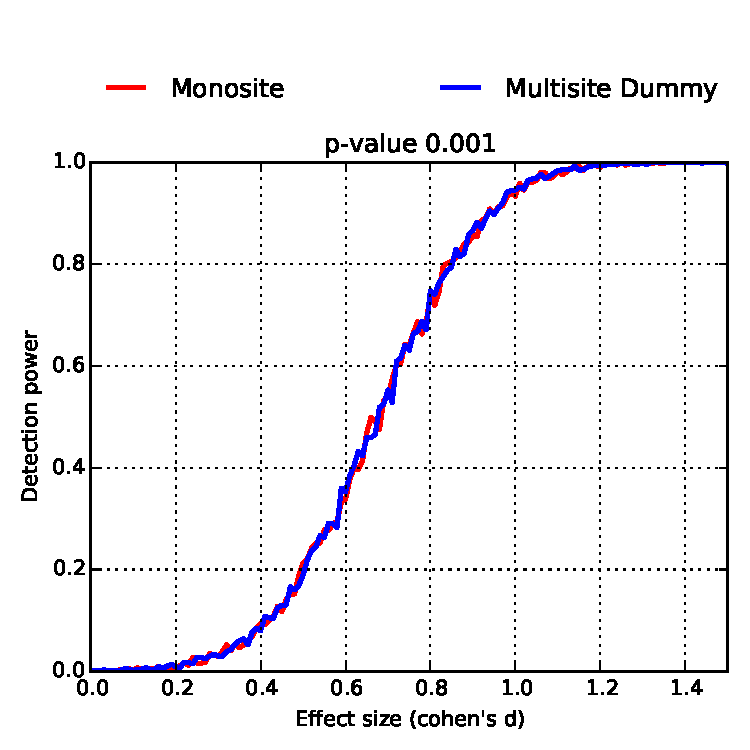
\includegraphics[width=0.39\textwidth]{../figures/detect_pow_bal5050_var0_site05.pdf}}\\[-2.7ex] 
     \hspace*{6.8em}
     \subfloat[\tiny Inter site-patho, no site effect]{ 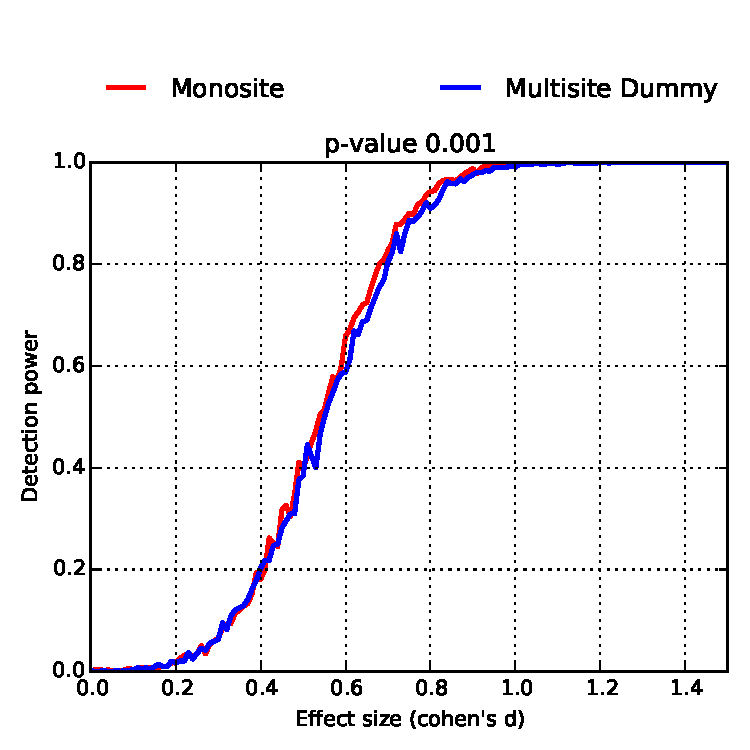
\includegraphics[width=0.39\textwidth]{../figures/detect_pow_bal5050_var2_site0.pdf}}
     \subfloat[\tiny Inter site-patho + site effect]{ 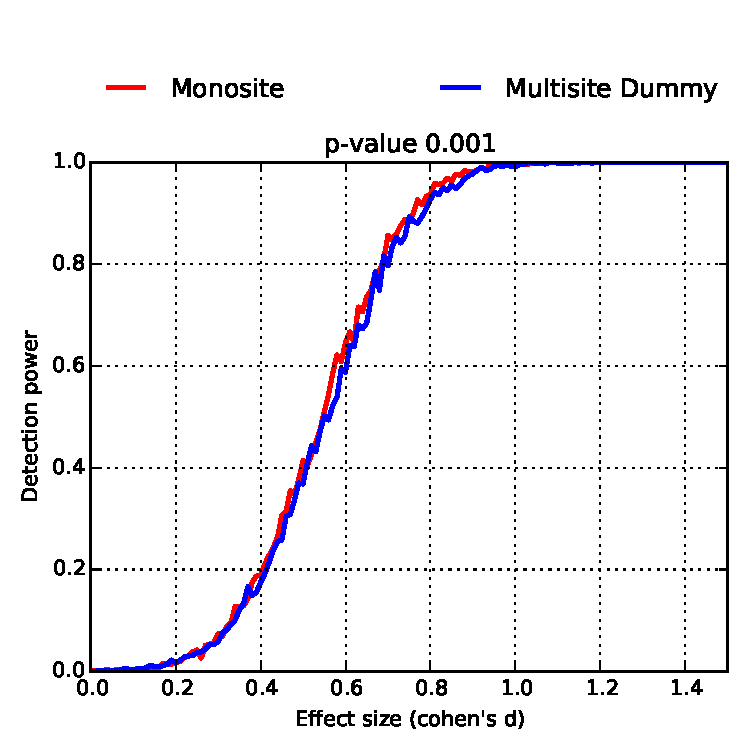
\includegraphics[width=0.39\textwidth]{../figures/detect_pow_bal5050_var2_site05.pdf}}\\
     \caption{
     Simulation of the detection power of two groups balanced 50\%-50\% between two sites. All plots show four scenarios in two configuration one monosite and two sites with correction for multisite differences using dummy variables. The first column represent scenarios without site effect and the second column show with a site effect the first row show simulation with out interaction site-pathology and the second row show with interaction.
}
\label{fig_full_sim_site_effect}
 \end{figure}
 

%
%\begin{frame} \frametitle{50-50 subjects, 70\%-30\% debalancing effect}
 \begin{figure}[tbp]
   \centering
    \captionsetup[subfloat]{labelformat=empty}
    \subfloat[]{ 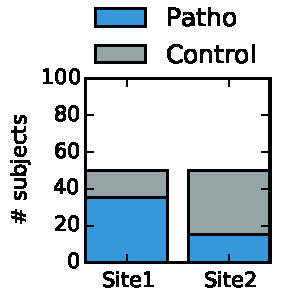
\includegraphics[width=0.19\textwidth]{../figures/prop_5050subj_7030.pdf}}
     \subfloat[\tiny No site effect]{\label{} 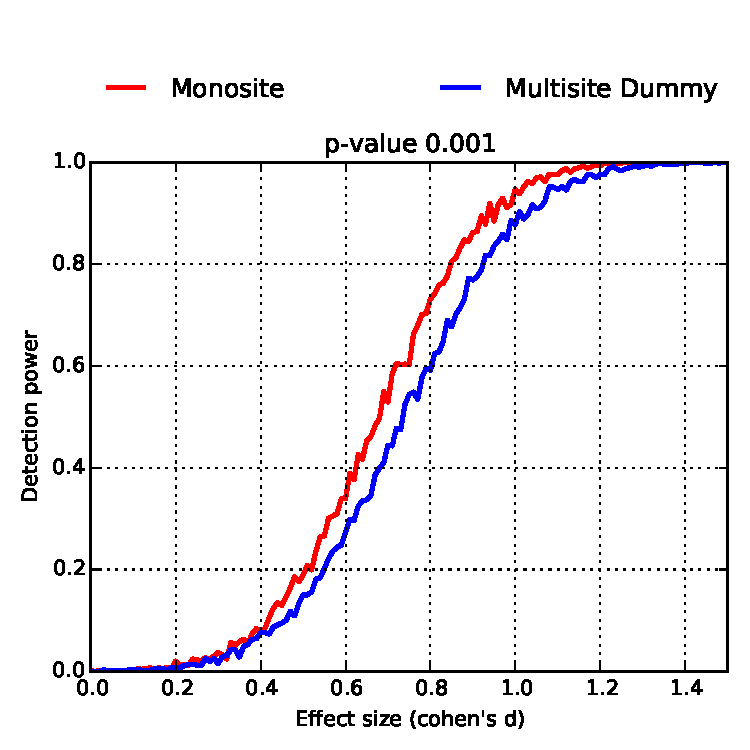
\includegraphics[width=0.39\textwidth]{../figures/detect_pow_bal7030_var0_site0.pdf}} 
     \subfloat[\tiny Site effect of 0.5]{\label{} 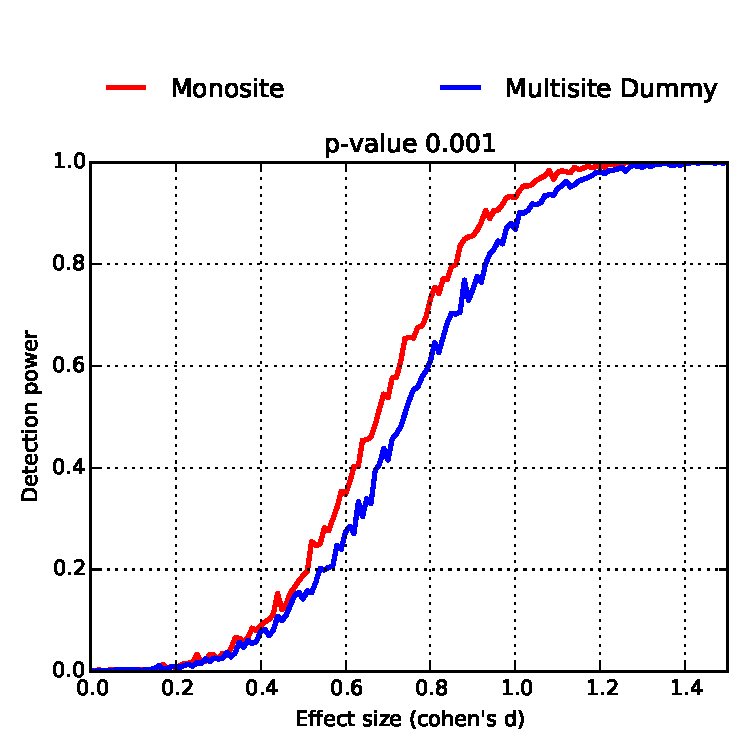
\includegraphics[width=0.39\textwidth]{../figures/detect_pow_bal7030_var0_site05.pdf}}\\[-2.7ex]
     \hspace*{6.8em}
     \subfloat[\tiny Interac site-patho, no site effect]{\label{} 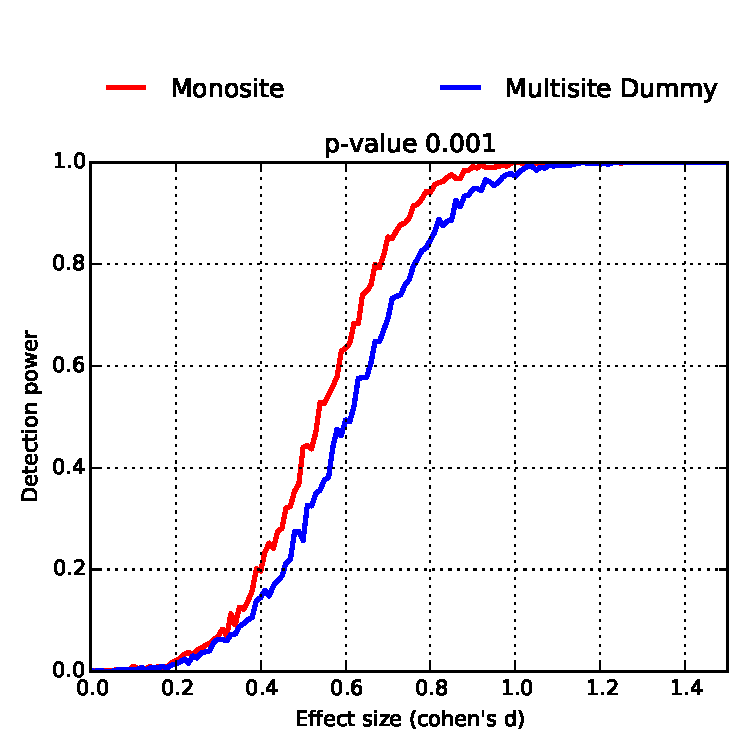
\includegraphics[width=0.39\textwidth]{../figures/detect_pow_bal7030_var2_site0.pdf}}
     \subfloat[\tiny Interac site-patho + site effect]{\label{} 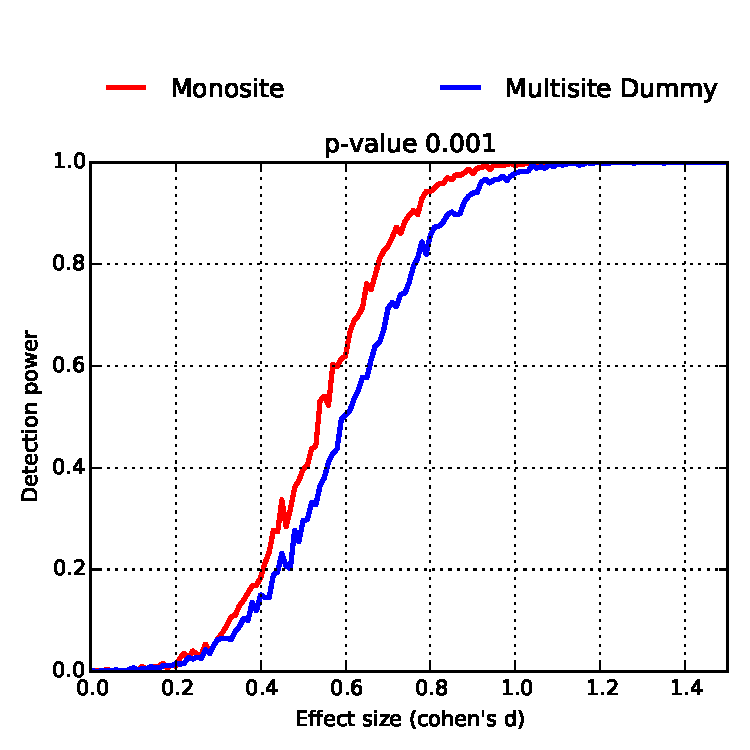
\includegraphics[width=0.39\textwidth]{../figures/detect_pow_bal7030_var2_site05.pdf}}\\
     \caption{
     Simulation of the detection power of two groups unbalanced 70\%-30\% between two sites. All plots show four scenarios in two configuration one monosite and two sites with correction for multisite differences using dummy variables. The first column represent scenarios without site effect and the second column show with a site effect the first row show simulation with out interaction site-pathology and the second row show with interaction.
}
     \label{fig_full_sim_debalancing}
 \end{figure}
 


%\frametitle{20-80 subjects, 50\%-50\% debalancing effect}
 \begin{figure}[tbp]
   \centering
    \captionsetup[subfloat]{labelformat=empty}
    \subfloat[]{ 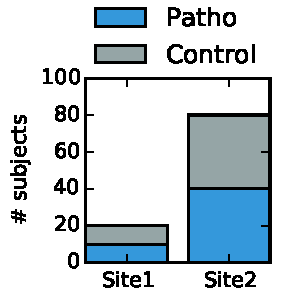
\includegraphics[width=0.19\textwidth]{../figures/prop_2080subj_5050.pdf}}
     \subfloat[\tiny No site effect]{\label{} 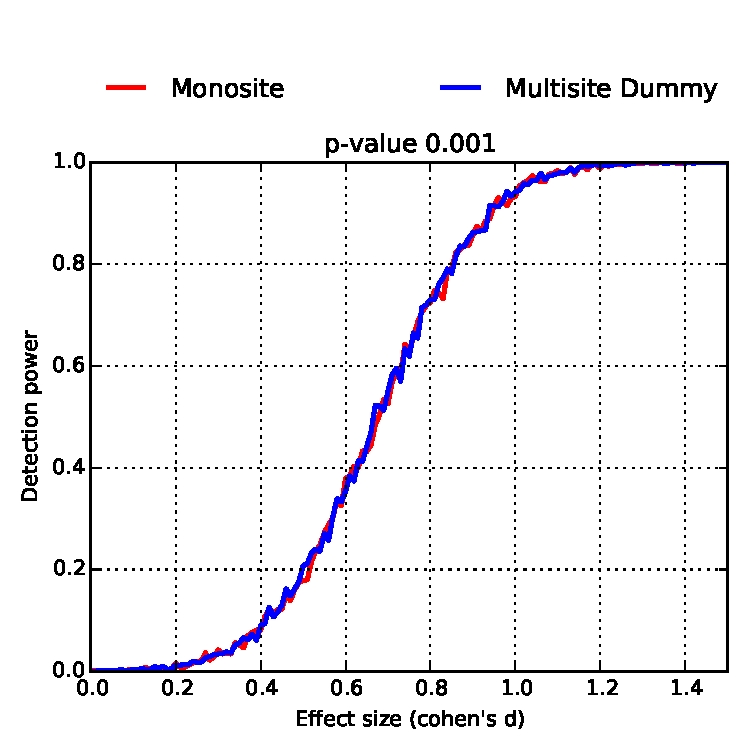
\includegraphics[width=0.39\textwidth]{../figures/detect_pow_2080bal5050_var0_site0.pdf}} 
     \subfloat[\tiny Site effect of 0.5]{\label{} 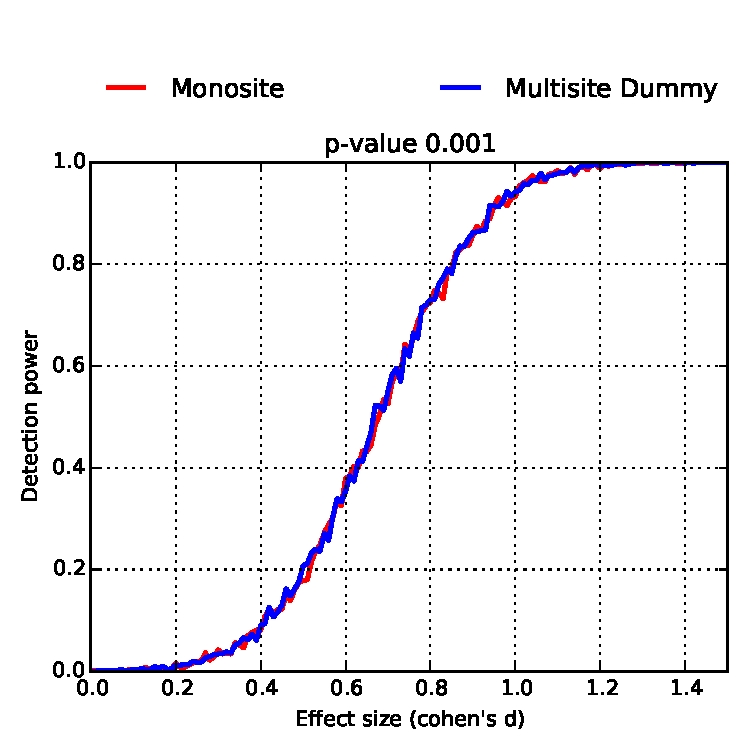
\includegraphics[width=0.39\textwidth]{../figures/detect_pow_2080bal5050_var0_site05.pdf}}\\[-2.7ex]
     \hspace*{6.8em}
     \subfloat[\tiny Interac site-patho, no site effect]{\label{} 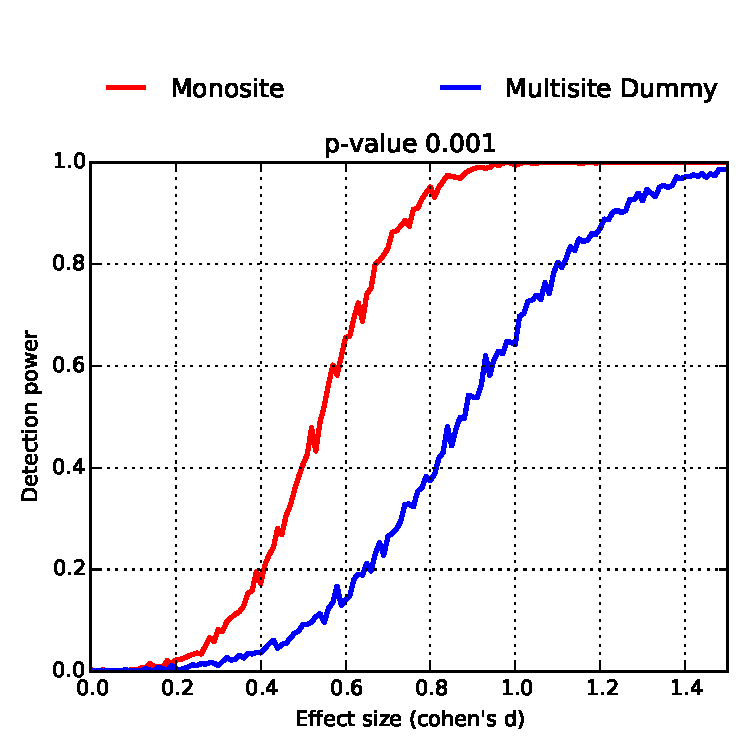
\includegraphics[width=0.39\textwidth]{../figures/detect_pow_2080bal5050_var2_site0.pdf}} 
     \subfloat[\tiny Interac site-patho + site effect]{\label{} 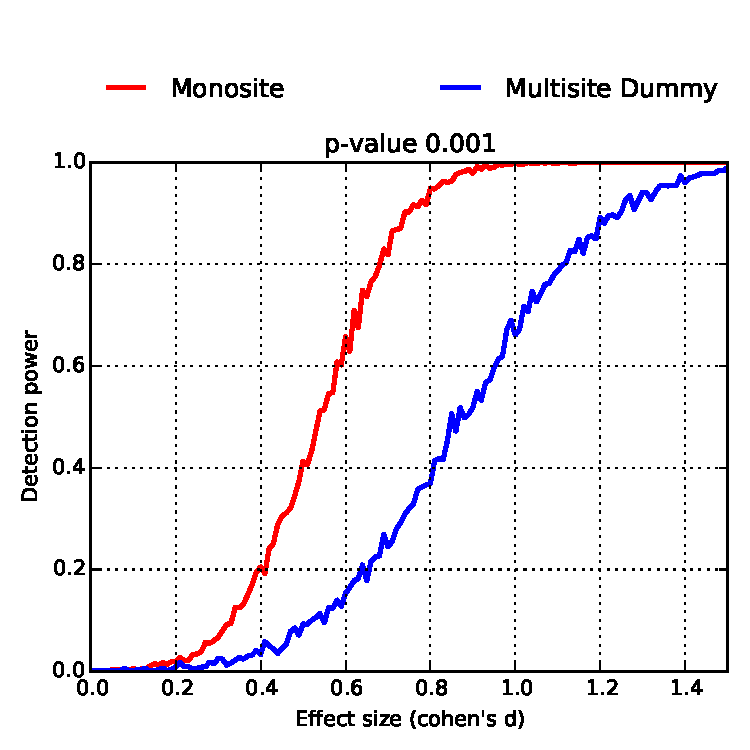
\includegraphics[width=0.39\textwidth]{../figures/detect_pow_2080bal5050_var2_site05.pdf}}\\
     \caption{
     Simulation of the detection power of two groups unbalanced 50\%-50\% between two sites, one small site of 20 subjects and one large of 80 subjects. All plots show four scenarios in two configuration one monosite and two sites with correction for multisite differences using dummy variables. The first column represent scenarios without site effect and the second column show with a site effect the first row show simulation with out interaction site-pathology and the second row show with interaction.
}
\label{fig_full_sim_2sites_balanced}
\end{figure}
 
Figure \ref{fig_full_sim_2sites_debalancing_inv} show the same configuration but the sample size are inverted. Has we can see we have the same pattern as in the real data with...

%\begin{frame} \frametitle{20-80 subjects, 70\%-30\% debalancing effect}
 \begin{figure}[tbp]
   \centering
    \captionsetup[subfloat]{labelformat=empty}
    \subfloat[]{ 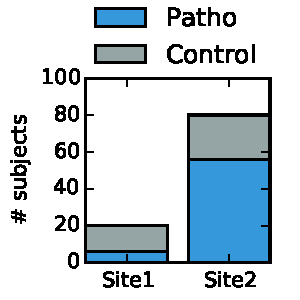
\includegraphics[width=0.19\textwidth]{../figures/prop_2080subj_7030.pdf}}
     \subfloat[\tiny No site effect]{\label{} 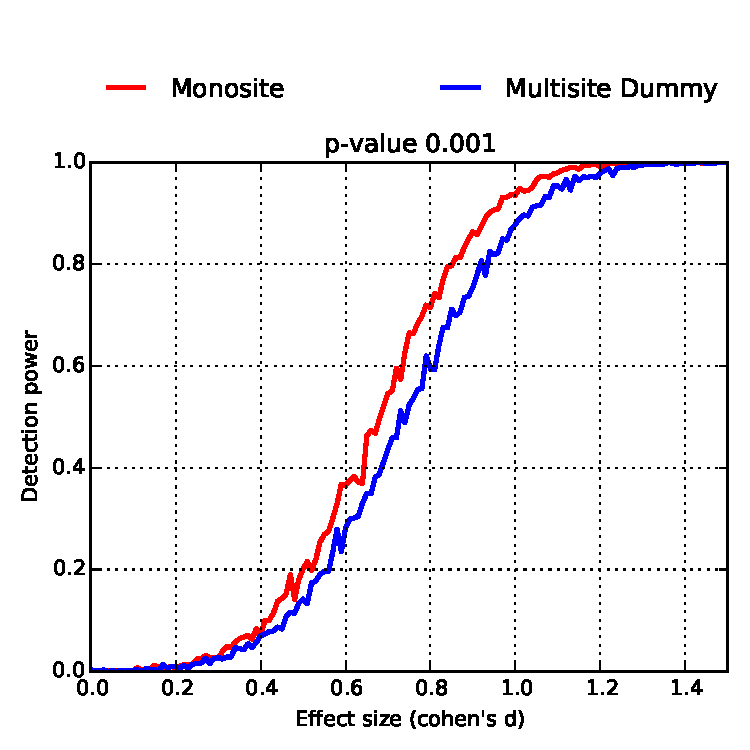
\includegraphics[width=0.39\textwidth]{../figures/detect_pow_2080bal7030_var0_site0.pdf}} 
     \subfloat[\tiny Site effect of 0.5]{\label{} 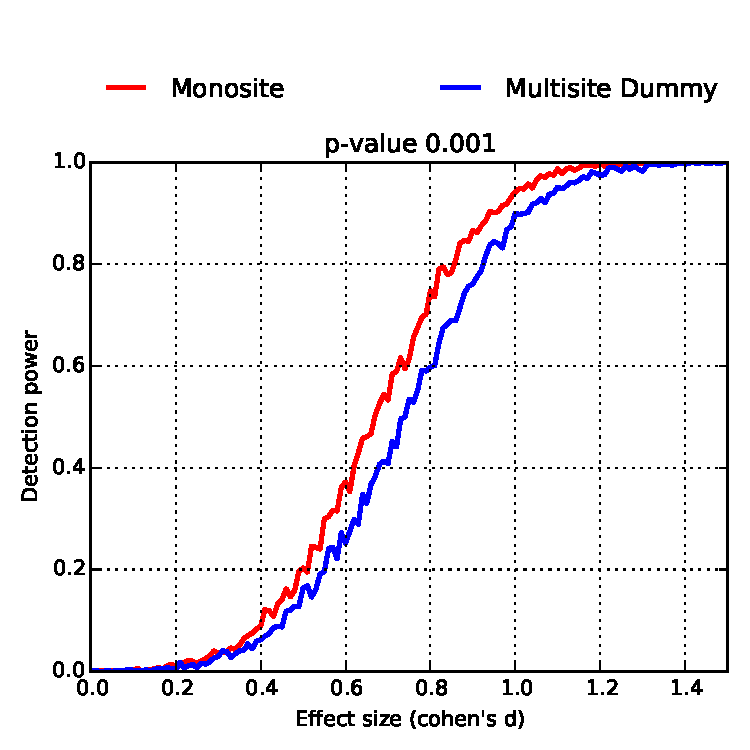
\includegraphics[width=0.39\textwidth]{../figures/detect_pow_2080bal7030_var0_site05.pdf}}\\[-2.7ex]
     \hspace*{6.8em}
     \subfloat[\tiny Interac site-patho, no site effect]{\label{} 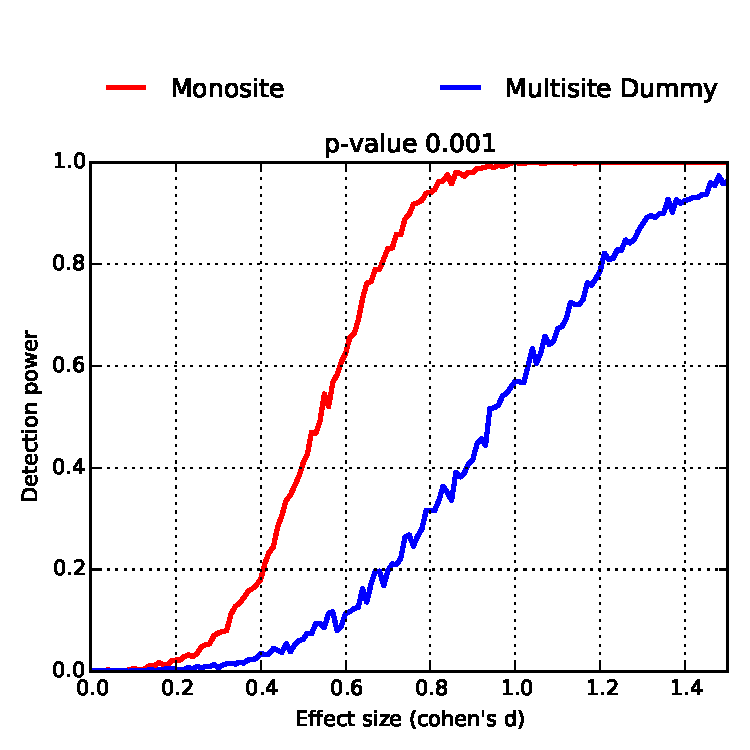
\includegraphics[width=0.39\textwidth]{../figures/detect_pow_2080bal7030_var2_site0.pdf}} 
     \subfloat[\tiny Interac site-patho + site effect]{\label{} 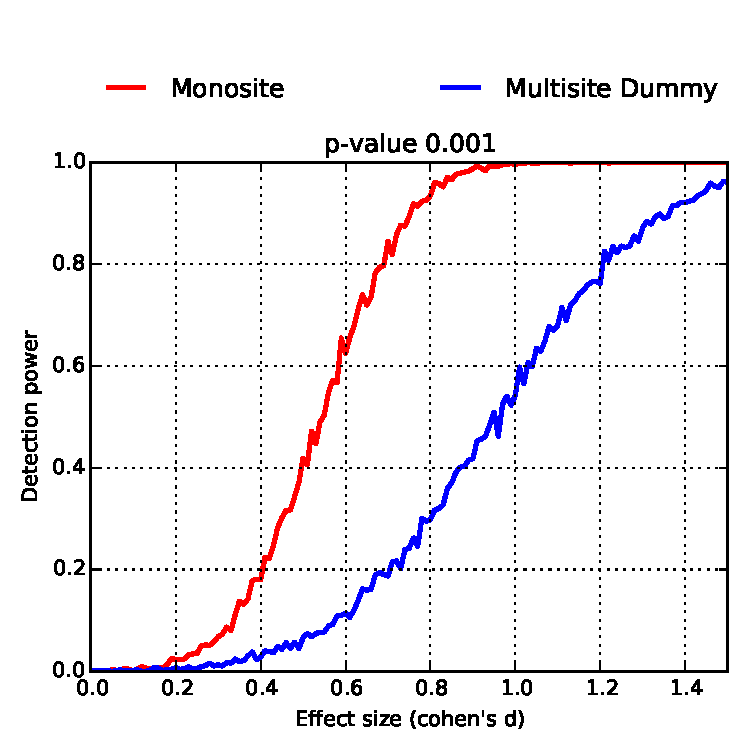
\includegraphics[width=0.39\textwidth]{../figures/detect_pow_2080bal7030_var2_site05.pdf}}\\
     \caption{
     Simulation of the detection power of two groups unbalanced 70\%-30\% between two sites, one small site of 20 subjects and one large of 80 subjects. All plots show four scenarios in two configuration one monosite and two sites with correction for multisite differences using dummy variables. The first column represent scenarios without site effect and the second column show with a site effect the first row show simulation with out interaction site-pathology and the second row show with interaction.
}
     \label{fig_full_sim_2sites_debalancing}
 \end{figure}
 
 


%\begin{frame} \frametitle{80-20 subjects, 70\%-30\% debalancing effect}
 \begin{figure}[tbp]
   \centering
    \captionsetup[subfloat]{labelformat=empty}
    \subfloat[]{ 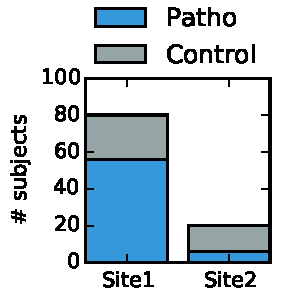
\includegraphics[width=0.19\textwidth]{../figures/prop_8020subj_7030.pdf}}
     \subfloat[\tiny No site effect]{\label{} 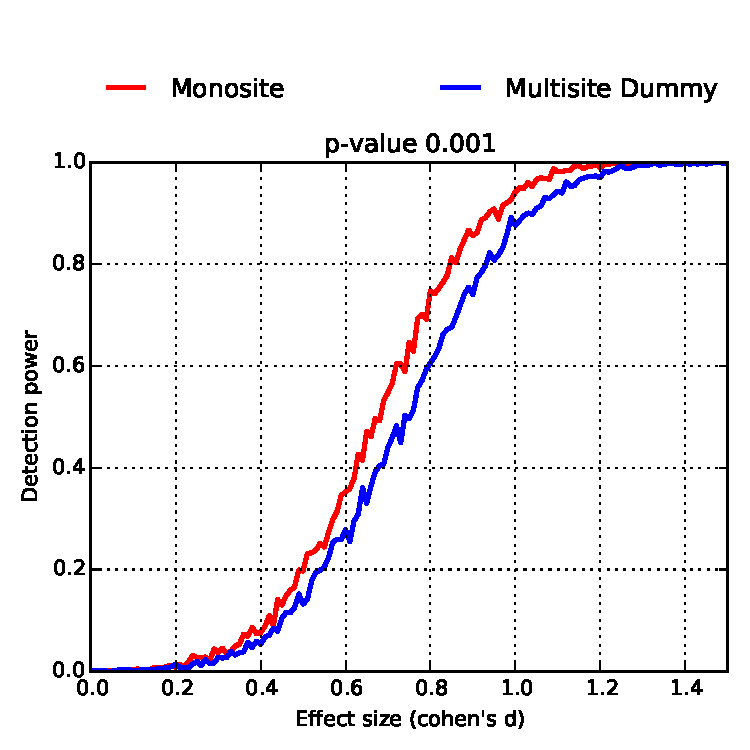
\includegraphics[width=0.39\textwidth]{../figures/detect_pow_8020bal7030_var0_site0.pdf}} 
     \subfloat[\tiny Site effect of 0.5]{\label{} 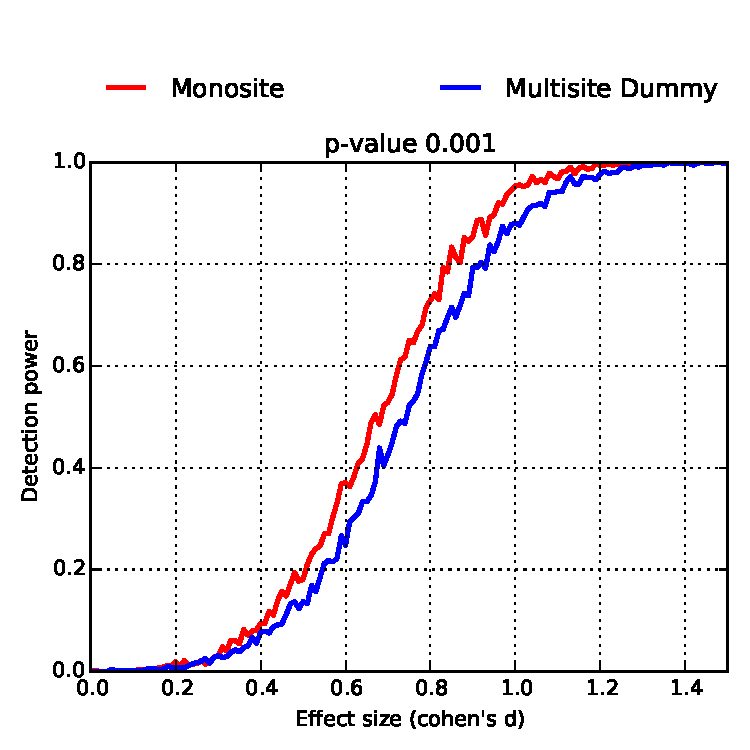
\includegraphics[width=0.39\textwidth]{../figures/detect_pow_8020bal7030_var0_site05.pdf}}\\[-2.7ex]
     \hspace*{6.8em}
     \subfloat[\tiny Interac site-patho, no site effect]{\label{} 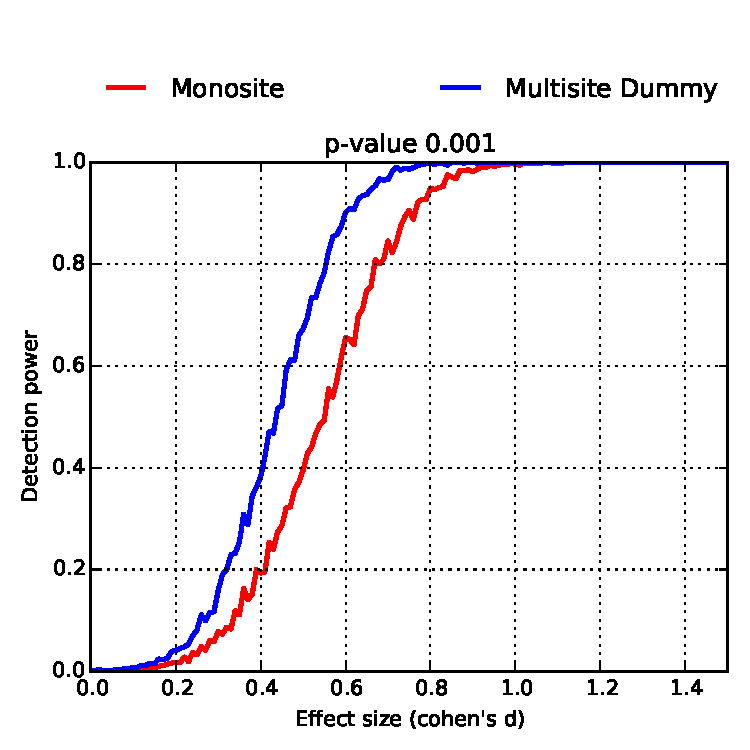
\includegraphics[width=0.39\textwidth]{../figures/detect_pow_8020bal7030_var2_site0.pdf}} 
     \subfloat[\tiny Interac site-patho + site effect]{\label{} 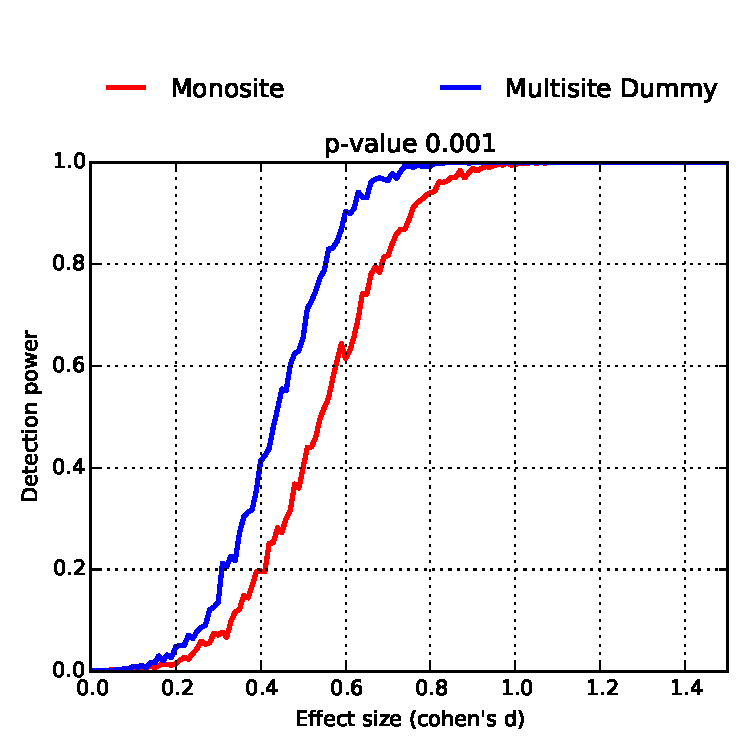
\includegraphics[width=0.39\textwidth]{../figures/detect_pow_8020bal7030_var2_site05.pdf}}\\
     \caption{
     Simulation of the detection power of two groups unbalanced 70\%-30\% between two sites, one small site of 20 subjects and one large of 80 subjects. All plots show four scenarios in two configuration one monosite and two sites with correction for multisite differences using dummy variables. The first column represent scenarios without site effect and the second column show with a site effect the first row show simulation with out interaction site-pathology and the second row show with interaction.
}
     \label{fig_full_sim_2sites_debalancing_inv}
 \end{figure}
 
Figure \ref{fig_full_sim_50sites_rnd_debalancing} show a more realistic case in clinical trials where the number of scanning sites is very large and the number of subjects per site is small. There is usually no control on the exact balancing of those sites therefore we have randomly assign debalancing for each site (between 10\% and 90\%) and have randomly assigned a number of subject to each site (between 2 and 15 subjects).

\begin{figure}[tbp]
   \centering
    \captionsetup[subfloat]{labelformat=empty}
     \subfloat[\tiny No interaction site-patho]{\label{} 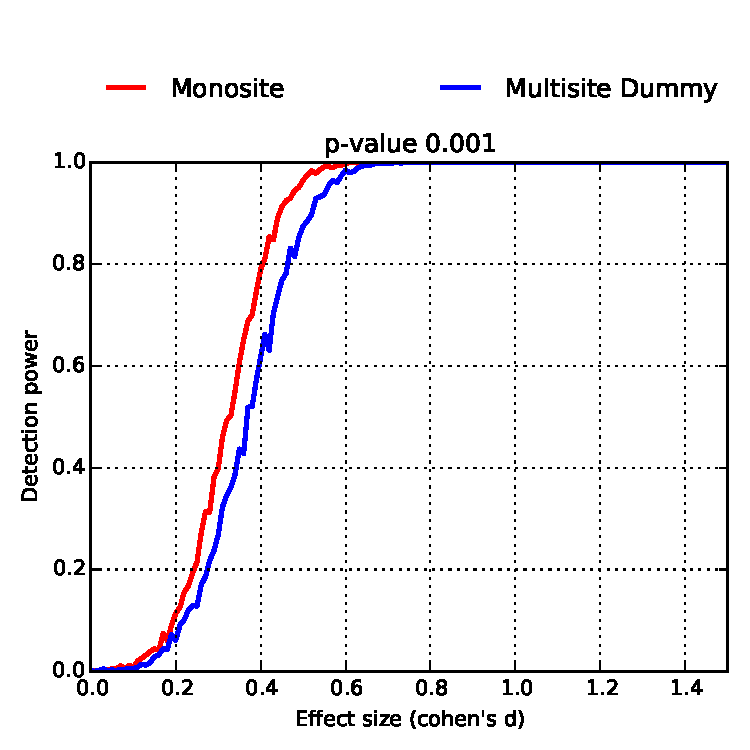
\includegraphics[width=0.39\textwidth]{../figures/detect_pow_rndsubj0215_50sites_rndbal1090_var0_siternd0005.pdf}} 
     \subfloat[\tiny Site effect of 0.5]{\label{} 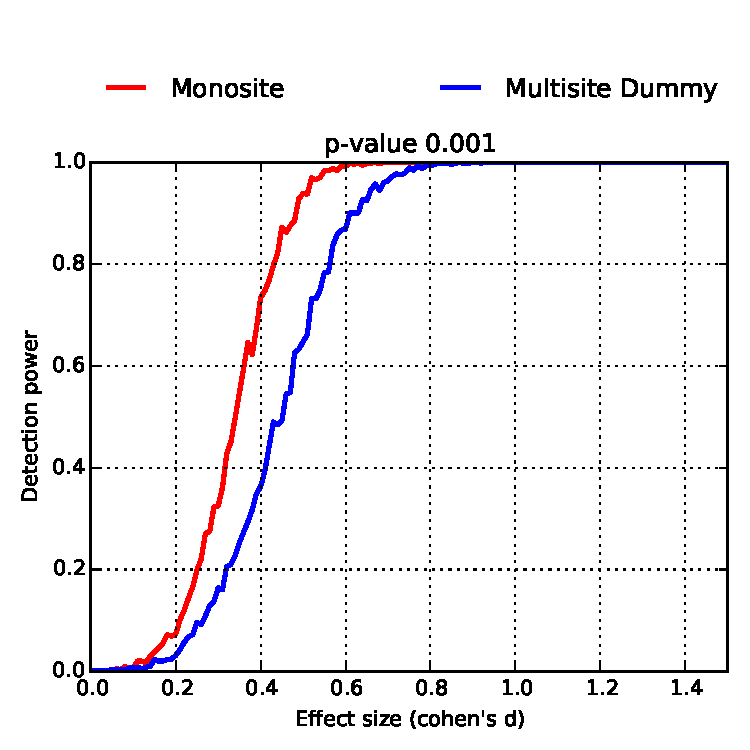
\includegraphics[width=0.39\textwidth]{../figures/detect_pow_rndsubj0215_50sites_rndbal1090_varrnd02_siternd0005.pdf}}\\
     \caption{
     Simulation of the detection power of two groups balanced randomly between 10\%-90\% between 50 sites, the number of subject per site is randomly assigned between 2 and 15. All plot show four scenario, one monosite and two sites with correction for multisite differences using dummy variables. The plots show the detection power when the variability is greater in one side then the other for the pathology group (twice the reference variability in one site and half the reference variability in the other one).
}
     \label{fig_full_sim_50sites_rnd_debalancing}
\end{figure}

\section{Discussion}

Connectivity bias that can impact interpretation.\\

Type of scanner most of them are Siemens we may have more variability if combining various brand\\

Talk about the impact in small acquisition 40 subjects total and the importance of pooling data among PI.\\

Talk about the impact in clinical trial and best practice.\\
	most of the time we cannot correct for site with one population only or with too few subjects per site. Although these kind of multisite studies generally sum-up to large dataset of more than 200 subjects. has we demonstrated in the synthetic simulation such configuration are comparable to single site analysis for this range of sample size.

It is better to have interaction of various amplitude across small sites than an average interaction on one large site\\

\section{Conclusion}


\section{Acknowledgments}
Parts of this work were presented at the 2013 annual meetings of the organization for human brain mapping \citep{Dansereau2013a}, as well as the  Alzheimer's Association International Conference (AAIC) (2013) (Boston) \citep{Dansereau2013b}. The authors are grateful to the members of the 1000 functional connectome consortium for publicly releasing there dataset. The computational resources used to perform the data analysis were provided by ComputeCanada\footnote{\url{https://computecanada.org/}} and CLUMEQ\footnote{\url{http://www.clumeq.mcgill.ca/}}, which is funded in part by NSERC (MRS), FQRNT, and McGill University. This project was funded by NSERC grant number RN000028, a salary award from ``Fonds de recherche du Qu\'ebec -- Sant\'e'' to PB as well as a salary award by the Canadian Institute of Health Research to CD.

\section*{References}

\bibliographystyle{elsarticle-harv}
\bibliography{cdansereau}


\pagebreak



\clearpage
\appendix


%% SUPPLEMENTARY MATERIAL
\clearpage
\pagebreak
\renewcommand{\thefigure}{S\arabic{figure}}
\renewcommand{\thetable}{S\arabic{table}}
\setcounter{figure}{0}
\begin{center}
\emph{Supplementary Material {--} Feasibility of multi-centric fMRI connectivity studies of Alzheimer's disease}\\

\vspace{\baselineskip}Submitted to Neuroimage.\\

\vspace{\baselineskip}C. Dansereau$^{1,2}$,  C. Risterucci$^{3}$, E. Merlo Pich$^{3}$, D. Arnold$^{4}$, P. Bellec$^{1,2}$\\

\end{center}
$^1$Functional Neuroimaging Unit, Centre de Recherche de l'Institut Universitaire de G\'eriatrie de Montr\'eal\\
$^2$Department of Computer Science and Operations Research, University of Montreal, Montreal, Quebec, Canada\\
$^3$F. Hoffmann-La Roche Ldt., Basel, Switzerland\\
$^4$NeuroRx, Montreal, Quebec, Canada\\

For all questions regarding the paper, please address correspondence to Pierre Bellec, CRIUGM, 4545 Queen Mary, Montreal, QC, H3W 1W5, Canada. Email: pierre.bellec (at) criugm.qc.ca.\\

\section*{Literature review: Alzheimer’s disease and resting-state fMRI} 
\begin{itemize}
\item \cite{Zhang2009a} used functional connectivity maps with a seed in the posterior cingulate cortex (PCC) to explore the differences between a group of elderly cognitively normal subjects (CNE, n=16) and patients with a mild dementia of the Alzheimer’s type (DAT, n=18).

\item \cite{Zhang2010} generalized the \cite{Zhang2009a} study with CNE (n=16) and a larger group of patients with DAT (n=46). Patients were separated in three groups (mild, moderate, severe DAT), and each group of patients was contrasted against the CNE.
\item \cite{Wang2006a} used functional connectivity maps with a seed in the hippocampi to explore the differences between a group of CNE (n=13) and patients with a mild DAT (n=13). All results included in the meta-analysis are from Table 2, seeded in the right hippocampus. Seeds were manually delineated on an individual basis.
\item \cite{Wang2007a} used functional connectivity maps with a seed in the posterior cingulate cortex (PCC) as well as full brain point-to-point correlations (based on an AAL parcellation) to explore the differences between a group of elderly cognitively normal subjects (CNE, n=14) and patients with a very mild to mild dementia of the Alzheimer’s type (DAT, n=14). Only the results based on the PCC seed were included in the meta-analysis.
\item \cite{Goveas2011} used functional connectivity maps with a seed in the hippocampi to explore the differences between a group of elderly cognitively normal subjects (CNE, n=18) and patients with a mild dementia of the Alzheimer’s type (DAT, n=14) before and after donepezil treatment. Seeds were manually delineated on an individual basis, before and after treatment.
\item \cite{Damoiseaux2012} used dual-regression independent component analysis to explore longitudinal differences between a group of CNE (n=18) and patients with DAT (n=21). All results included in the meta-analysis are from Table 3 (differences at baseline) and Table 4 (interaction with time). The authors used three components representing the Anterior DMN, Ventral DMN and Posterior DMN.
\end{itemize}


\pagebreak
% 
% \begin{figure}[!ht]
% \begin{center}
% 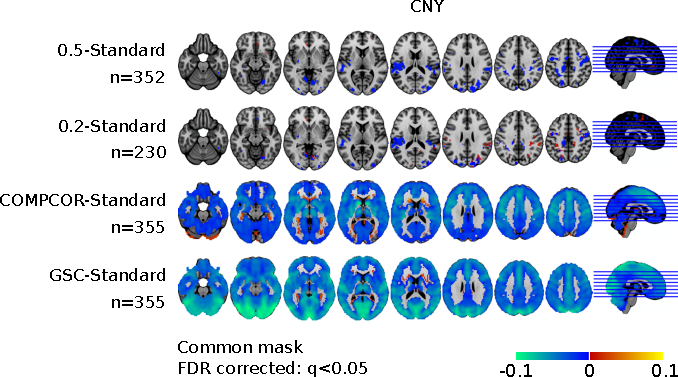
\includegraphics[width=\linewidth]{../figures/figure_comp_cny.pdf}
% \end{center}
% \caption{
% {\bf Differences in functional connectivity for the default mode network (seed in the PCC). Differences in connectivity between all the CNY with scrubbing ($FD>0.5$ and $FD>0.2$), CompCor, and GSC. The mask used depict only significant result of the $t$-test (FDR correction $q<0.05$) only the two scrubbing procedures use the union of there respective mask (common mask).}
% }
% \label{fig_sup_scrubbimpact_cny}
% \end{figure}
% 
% \begin{figure}[!ht]
% \begin{center}
% 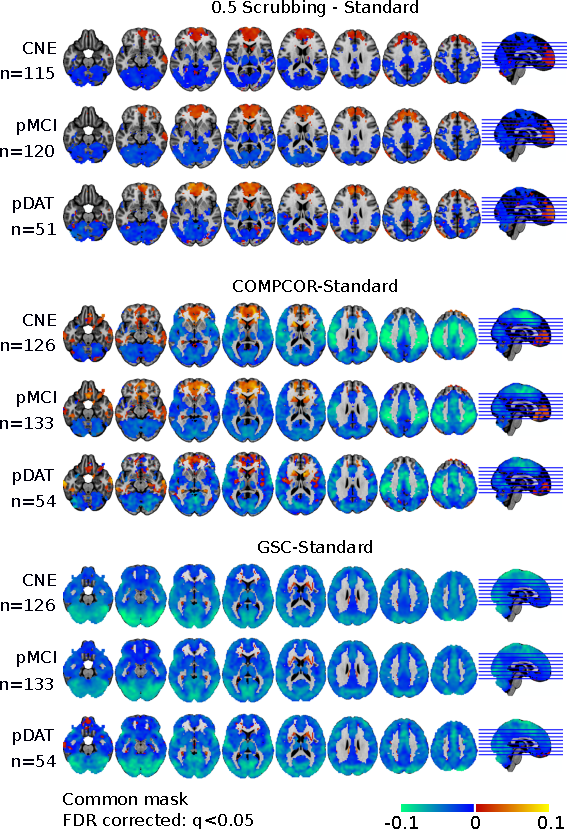
\includegraphics[width=0.75\linewidth]{../figures/scrubbing_impact_cne_mci_dat_all.pdf}
% \end{center}
% \caption{
% {\bf Differences in functional connectivity for the default mode network (seed in the PCC). Differences in connectivity for each group (CNE, pMCI, pDAT) compared to basedline (standard preprocessing) with and without scrubbing ($FD>0.5$ and $FD>0.2$) (FDR correction $q<0.05$) for all voxels showing a significant effect in at least one of the contrast.}
% }
% \label{fig_sup_impact_on_groups}
% \end{figure}



%\frametitle{Inter-site vs intra-site variability}
% \begin{figure}[H]
% \begin{center}
% 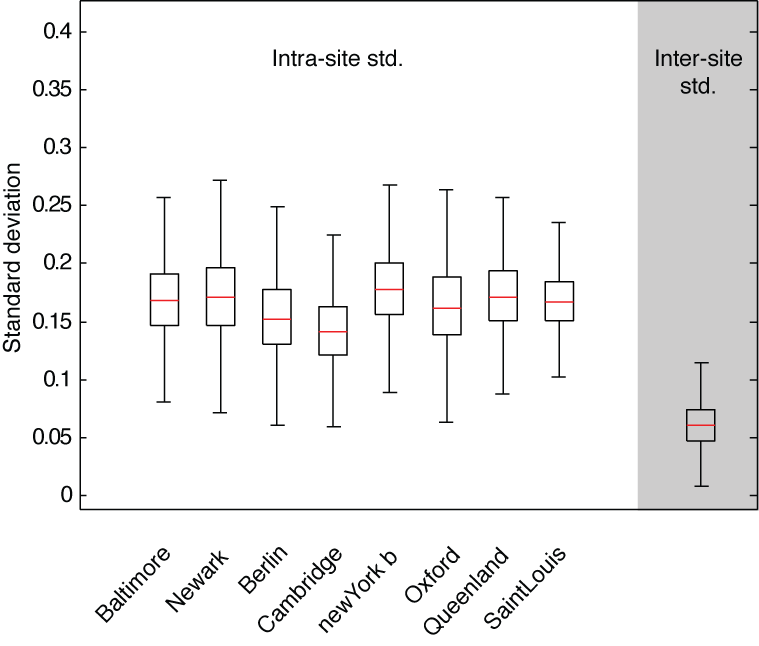
\includegraphics[width=0.6\linewidth]{../figures/inter_vs_intra_3tonly.png}
% \end{center}
% \tiny{Dansereau et al. manuscript in preparation}
% \end{figure}
% 





% \begin{table}[!ht]
% \begin{center}
% \includegraphics[width=\linewidth]{../figures/tab_fdr.pdf}
% \end{center}
% \caption{
% {\bf Summary of the empirical false-discovery rate of GLM-connectome (with group or BH FDR), NBS and MDMR on simulations.} {Etc.} 
% }
% \label{tab_fdr}
% \end{table}



\end{document}


